\part{Outlook for CLFV Searches Using Top Quarks}
\label{Part4}
\autoref{Part4} of this thesis describes an ongoing physics analysis that is an extension of the analysis documented in \autoref{Part3}. Under the supervision of Prof. Skinnari, Emily Minyun Tsai and I started working on this analysis in January 2023. Materials presented in \autoref{Part4} have not yet been fully approved by the \ac{CMS} Collaboration and shall not be considered to be finalized. \autoref{Part4} is organized as follows. \autoref{chap:Signal} gives a description of the signal processes targeted by this analysis and how they are generated. Object- and event-level selection criteria used by this analysis are described in \autoref{chap:Obj} and \autoref{chap:Evt}, respectively. \autoref{chap:Sensitivity} presents results of a preliminary sensitivity study. Except where noted, materials presented in \autoref{Part4} are prepared by Emily and myself.
\chapter{Inclusive CLFV Signals}
\label{chap:Signal}

As discussed in \autoref{chap:History}, the \ac{CLFV} processes involving top quarks have been studied by the \ac{ATLAS} and \ac{CMS} Collaborations in many orthogonal channels. Among all possible charged-lepton flavor mixing modes (i.e. e$\upmu$, e$\uptau$, and $\upmu\uptau$), the e$\upmu$ mode receives the most extensive scrutiny~\cite{ATLAS-CONF-2018-044,CMS:2022ztx,CMS:2023phe}, yielding a very tight constraint at $\mathcal{O}(10^{-8})$ on $\mathcal{B}(\tto{q})$. On the other hand, there exists only one \ac{ATLAS} study on the $\upmu\uptau$ mode~\cite{ATLAS-CONF-2023-001}, and the e$\uptau$ mode remains completely unexplored at the \ac{LHC} experiments. Therefore, the objective of this analysis is to probe as many unexplored channels as possible and search for all three charged-lepton flavor mixing modes simultaneously using data collected by the \ac{CMS} detector in 2016-2018. \autoref{sec:Target} gives a brief description of the targeted final states while signal event generation is described in \autoref{sec:SigGen}.
%%%%%%%%%%%%%%%%%%%%%%%%%%%%%%%%%%%%%%%%%%%
%%%%%%%%%%%%%%%%%%%%%%%%%%%%%%%%%%%%%%%%%%%
\section{Targeted Final States}
\label{sec:Target}

One of the central features of this analysis is the inclusion of hadronic tau lepton, which remains relatively unexplored in the top quark sector. The target final states of this analysis contain exactly two light leptons (electron or muon) and one hadronic tau. The two light leptons can come with any flavor- and charge-compositions, as long as the sum of the electric charges of all three leptons is 1 or -1. Effectively, this guarantees all three lepton flavor mixing modes are covered by this analysis. In addition to leptons, the target final states at \ac{LO} also feature one or two jets with exactly one jet originating from a b quark and some imbalances in $\pt$ caused by neutrinos. Representative Feynman diagrams are shown in Figure~\ref{fig:Target}.

 \begin{figure}[tbh!]
 \begin{center}
 \begin{tabular}{ccc}
 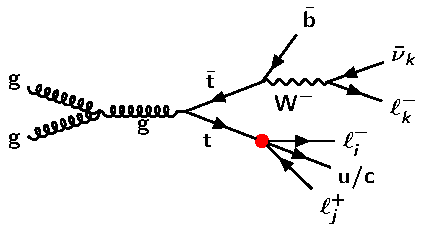
\includegraphics[width=0.33\textwidth]{figures/Part4/Signal/TT}&
 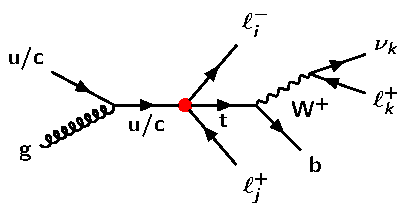
\includegraphics[width=0.33\textwidth]{figures/Part4/Signal/ST1}&
 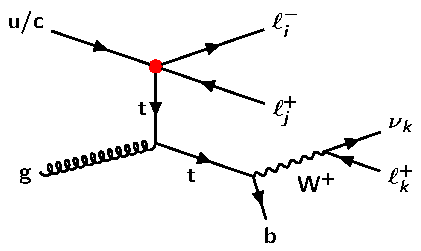
\includegraphics[width=0.33\textwidth]{figures/Part4/Signal/ST2}\\
 \end{tabular}
 \caption{Representative Feynman diagrams for the signal processes that are targeted by this analysis. Both top quark decay (left) and production (middle and right) \ac{CLFV} processes are shown. The indices $i$, $j$, and $k$ are lepton flavor indices that run from 1 to 3 with the following conditions: i) $i\neq j$, ii) one of these three indices is 3, and iii) the other two are smaller than 3.}
 \label{fig:Target}
 \end{center}
 \end{figure}

Even though the e$\upmu$ flavor mixing mode is covered by this analysis, the corresponding processes can only enter the event selection through the \ac{OS}-e$\upmu$ channel with a hadronic tau produced by the \ac{SM} top quark. Depending on the charge assignment, the same event topology may also contribute to the e$\uptau$ or $\upmu\uptau$ modes, as the hadronic tau may also come from the flavor-violating vertex. Furthermore, the e$\uptau$ and $\upmu\uptau$ signals can enter the event selection through \ac{SS} dilepton channels, where the background yields are much lower. Therefore, it is expected that this analysis is more competitive in its sensitivity on e$\uptau$ and $\upmu\uptau$ modes.
%%%%%%%%%%%%%%%%%%%%%%%%%%%%%%%%%%%%%%%%%%%
%%%%%%%%%%%%%%%%%%%%%%%%%%%%%%%%%%%%%%%%%%%
\section{Signal Event Generation}
\label{sec:SigGen}

In general, the strategy to generate the \ac{CLFV} signal events for this analysis is very similar to the existing strategy described in \autoref{sec:Signals}. One notable distinction is that all three charged-lepton flavor mixing modes are enabled in samples produced for this analysis. This is achieved by explicitly turning on the e$\uptau$ and $\upmu\uptau$ terms in the \ac{EFT} operators. For example, the parameterization of the scalar-like operator specified in Equation~\ref{eq:1:4} is modified as,

\begin{eqnarray}
\textsf{C}_{\textsf{lequ}}^{(1)}  
 &=& \textsf{C}_{\textsf{lequ}}^{(1)1213}
 + \textsf{C}_{\textsf{lequ}}^{(1)2113}
 + \textsf{C}_{\textsf{lequ}}^{(1)1231}
 + \textsf{C}_{\textsf{lequ}}^{(1)2131} \nonumber\\
 &+& \textsf{C}_{\textsf{lequ}}^{(1)1313}
 + \textsf{C}_{\textsf{lequ}}^{(1)3113}
 + \textsf{C}_{\textsf{lequ}}^{(1)1331}
 + \textsf{C}_{\textsf{lequ}}^{(1)3131} \\
 &+& \textsf{C}_{\textsf{lequ}}^{(1)2313}
 + \textsf{C}_{\textsf{lequ}}^{(1)3213}
 + \textsf{C}_{\textsf{lequ}}^{(1)2331}
 + \textsf{C}_{\textsf{lequ}}^{(1)3231}. \nonumber
\label{eq:example}
\end{eqnarray}

This is only done to simplify the \ac{MC} production procedure as the number of unique samples can be reduced by a factor of three. From a theoretical point of view, each flavor mixing mode corresponds to an independent \ac{WC} without any presumed correlations with other \acp{WC}. The generated signal events from one sample are therefore categorized into three groups using information at the generator level. Since the lepton masses are neglected in the \ac{ME} calculation, the theoretical cross-section is identical across different flavor mixing modes. Therefore, events from all three groups are normalized to the same cross-section listed in Table~\ref{tab:signal}. 

The effective Lagrangian is implemented using the SMEFTsim~\cite{Brivio:2017btx} model, which is the common standard agreed by the \ac{ATLAS} and \ac{CMS} Collaborations. Other than the differences in signal cross-sections reported by different models. The \ac{CKM} and \ac{PMNS} matrices are also treated differently by SmeftFR~\cite{Dedes:2019uzs} and SMEFTsim. More specifically, nonzero off-diagonal terms are added to the entries of the \ac{CKM} and \ac{PMNS} matrices by SmeftFR while both matrices are set to identity by SMEFTsim. Effectively, this means SMEFTsim allows no contributions from \acp{FCCC} to the signal processes. Consequently, this results in a softer kinematic distribution of final-state particles even though the difference is largely negligible, as is shown in Figure~\ref{fig:reweight}.

Generator-level leptons that emerge from the \ac{EFT} vertex are generally far more energetic in the top quark production events than the top quark decay events. This notable distinction between the two signal modes is exploited to benefit sensitivity, which is discussed in \autoref{sec:SRInclusive}. Representative kinematic distributions of the simulated signal events at the generator level are shown in Figure~\ref{fig:SigGen}.

 \begin{figure}[tbh!]
 \begin{center}
 \begin{tabular}{ccc}
 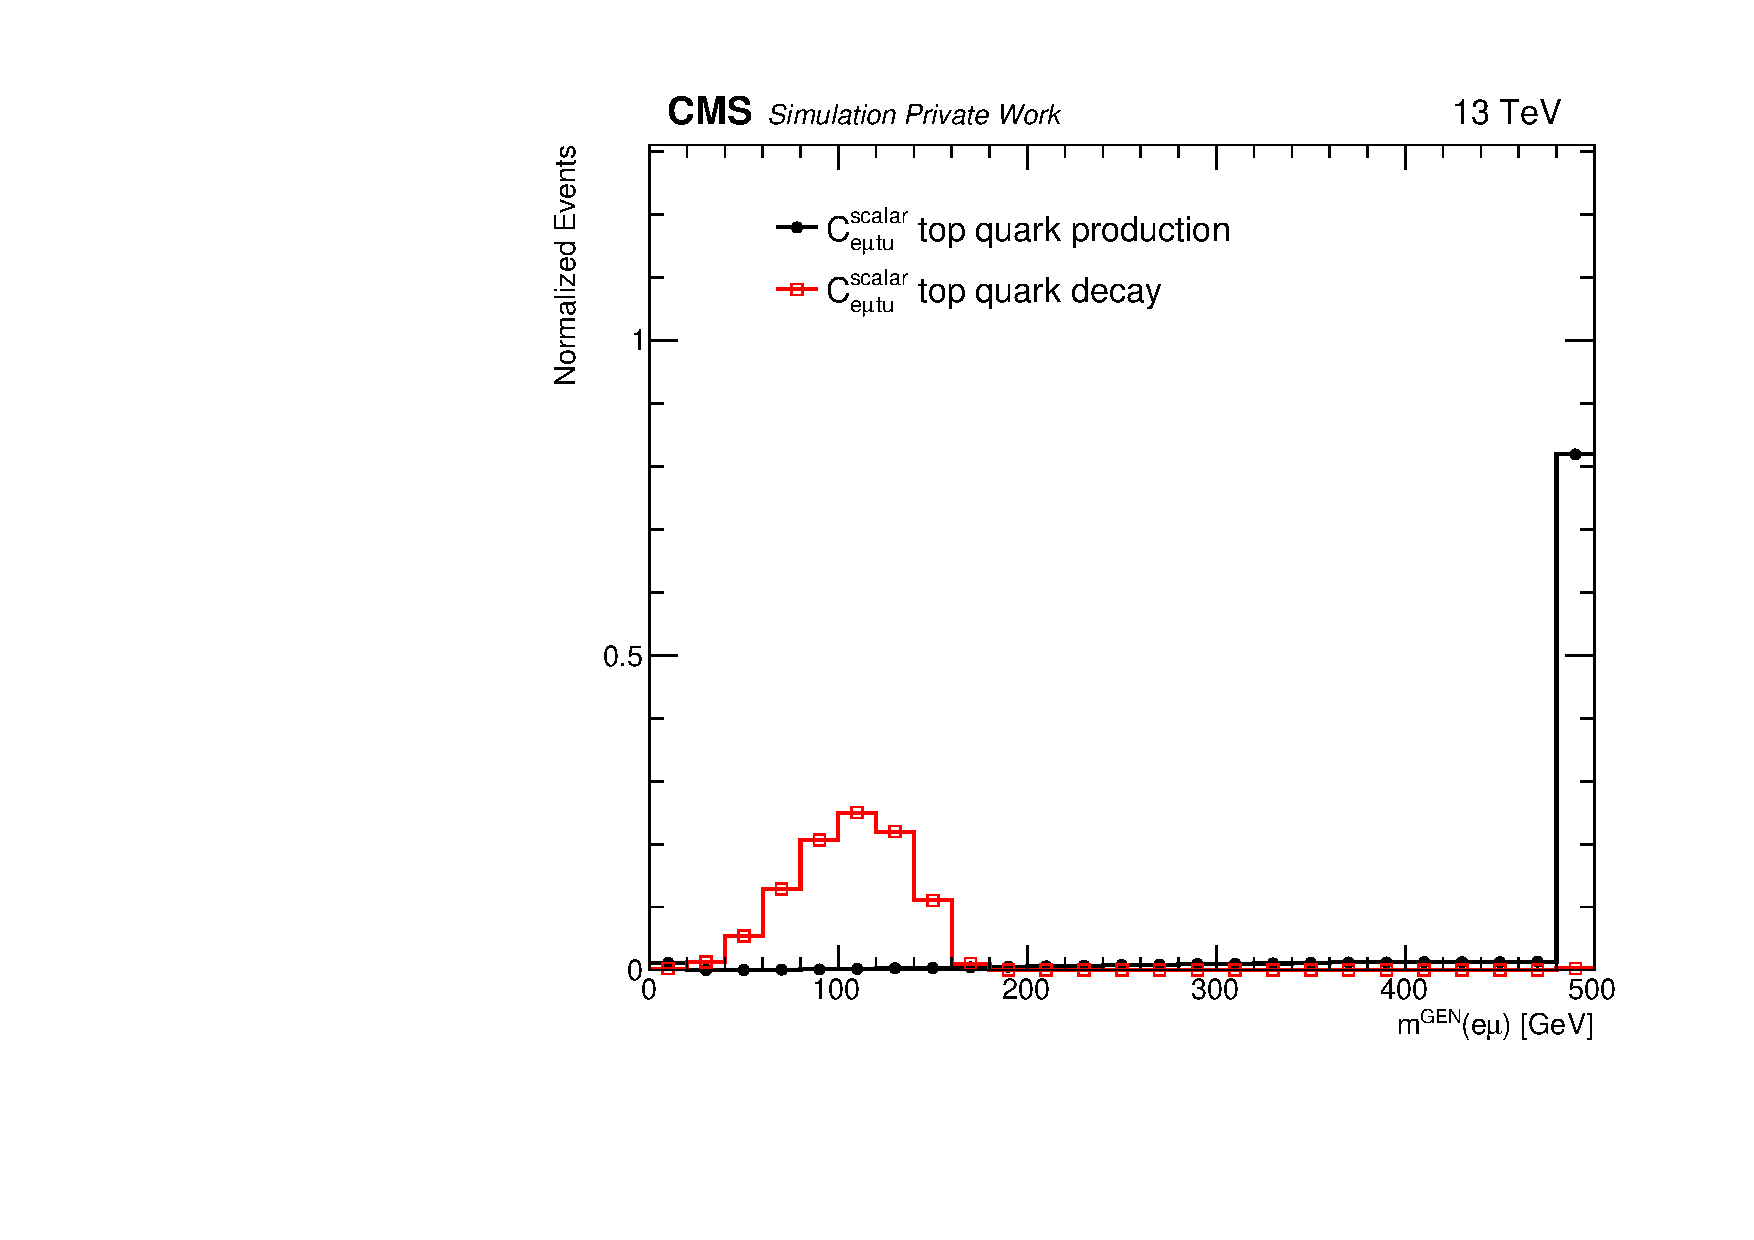
\includegraphics[width=0.33\textwidth]{figures/Part4/Signal/llM_emu}&
 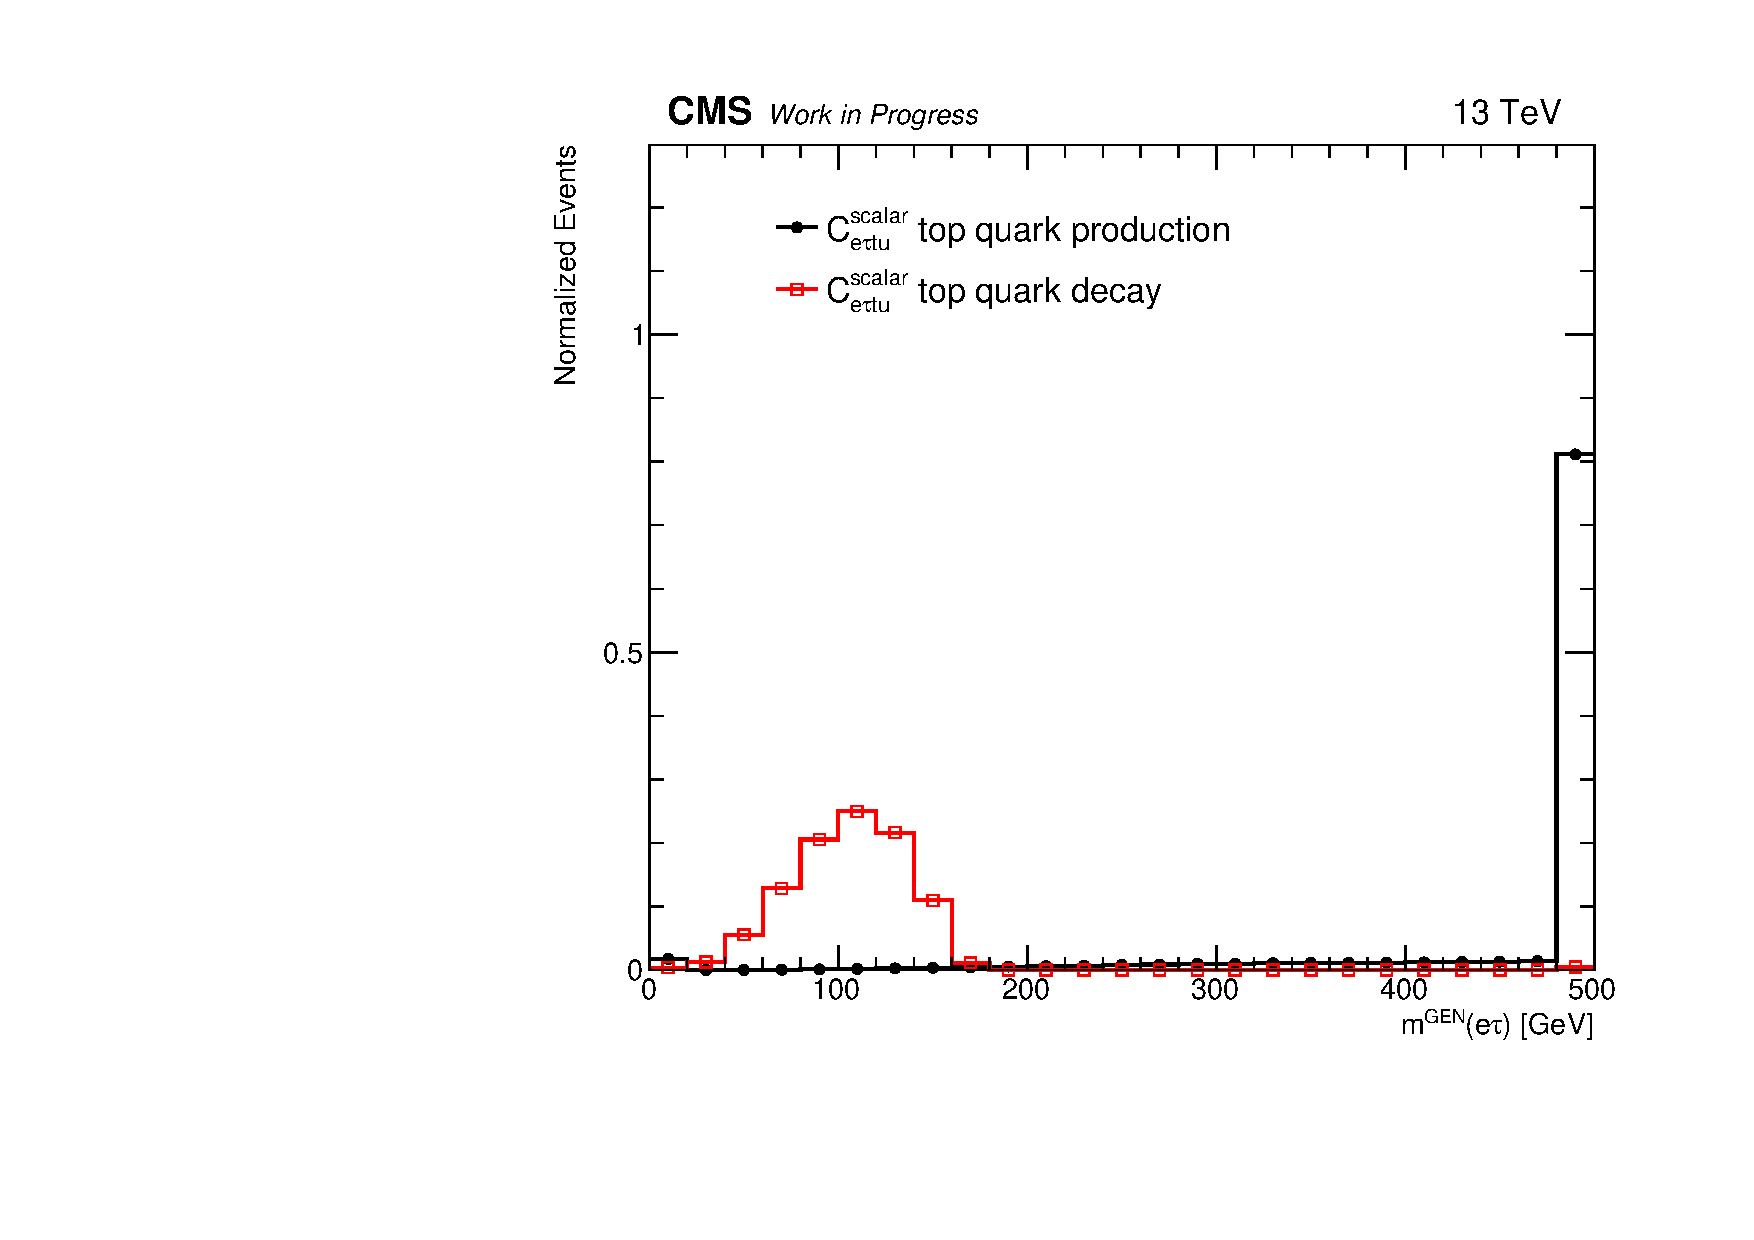
\includegraphics[width=0.33\textwidth]{figures/Part4/Signal/llM_etau}&
 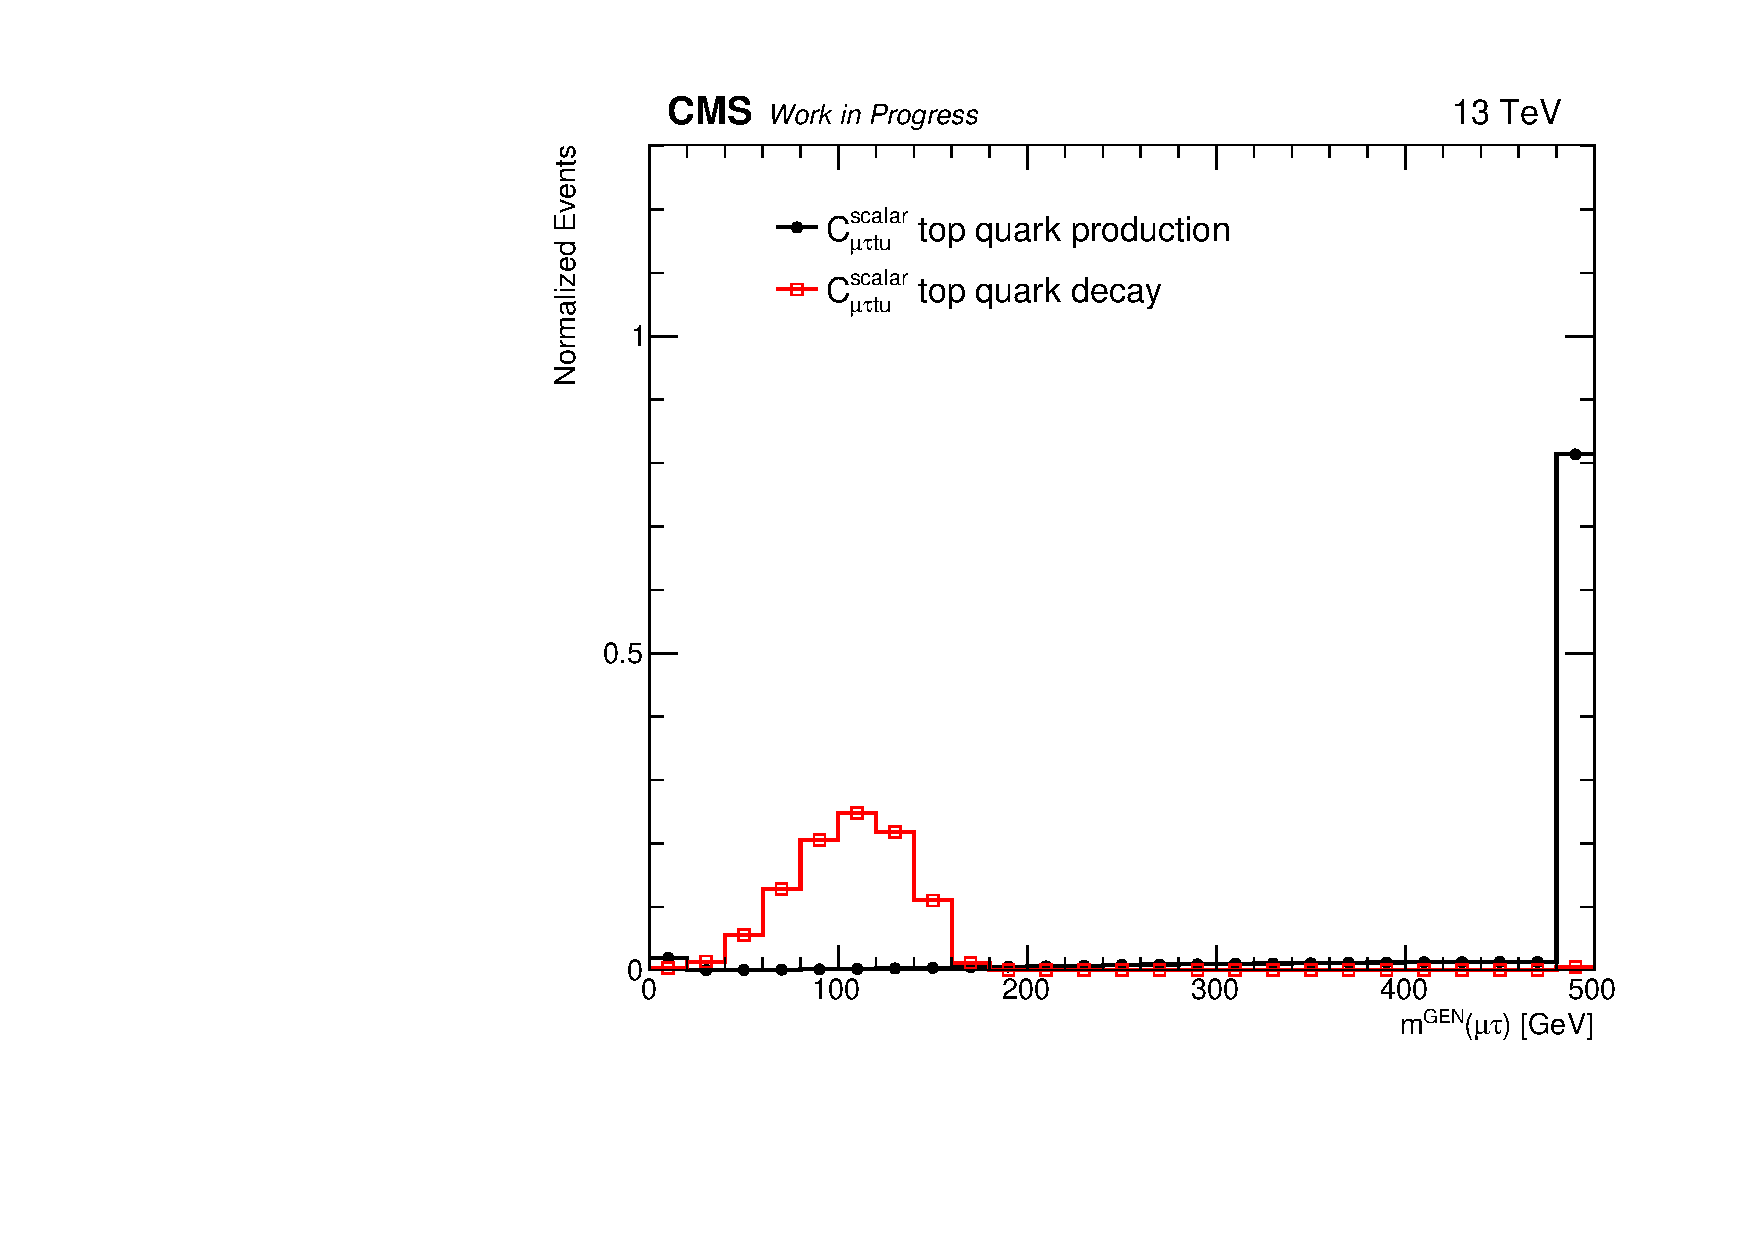
\includegraphics[width=0.33\textwidth]{figures/Part4/Signal/llM_mutau}\\
 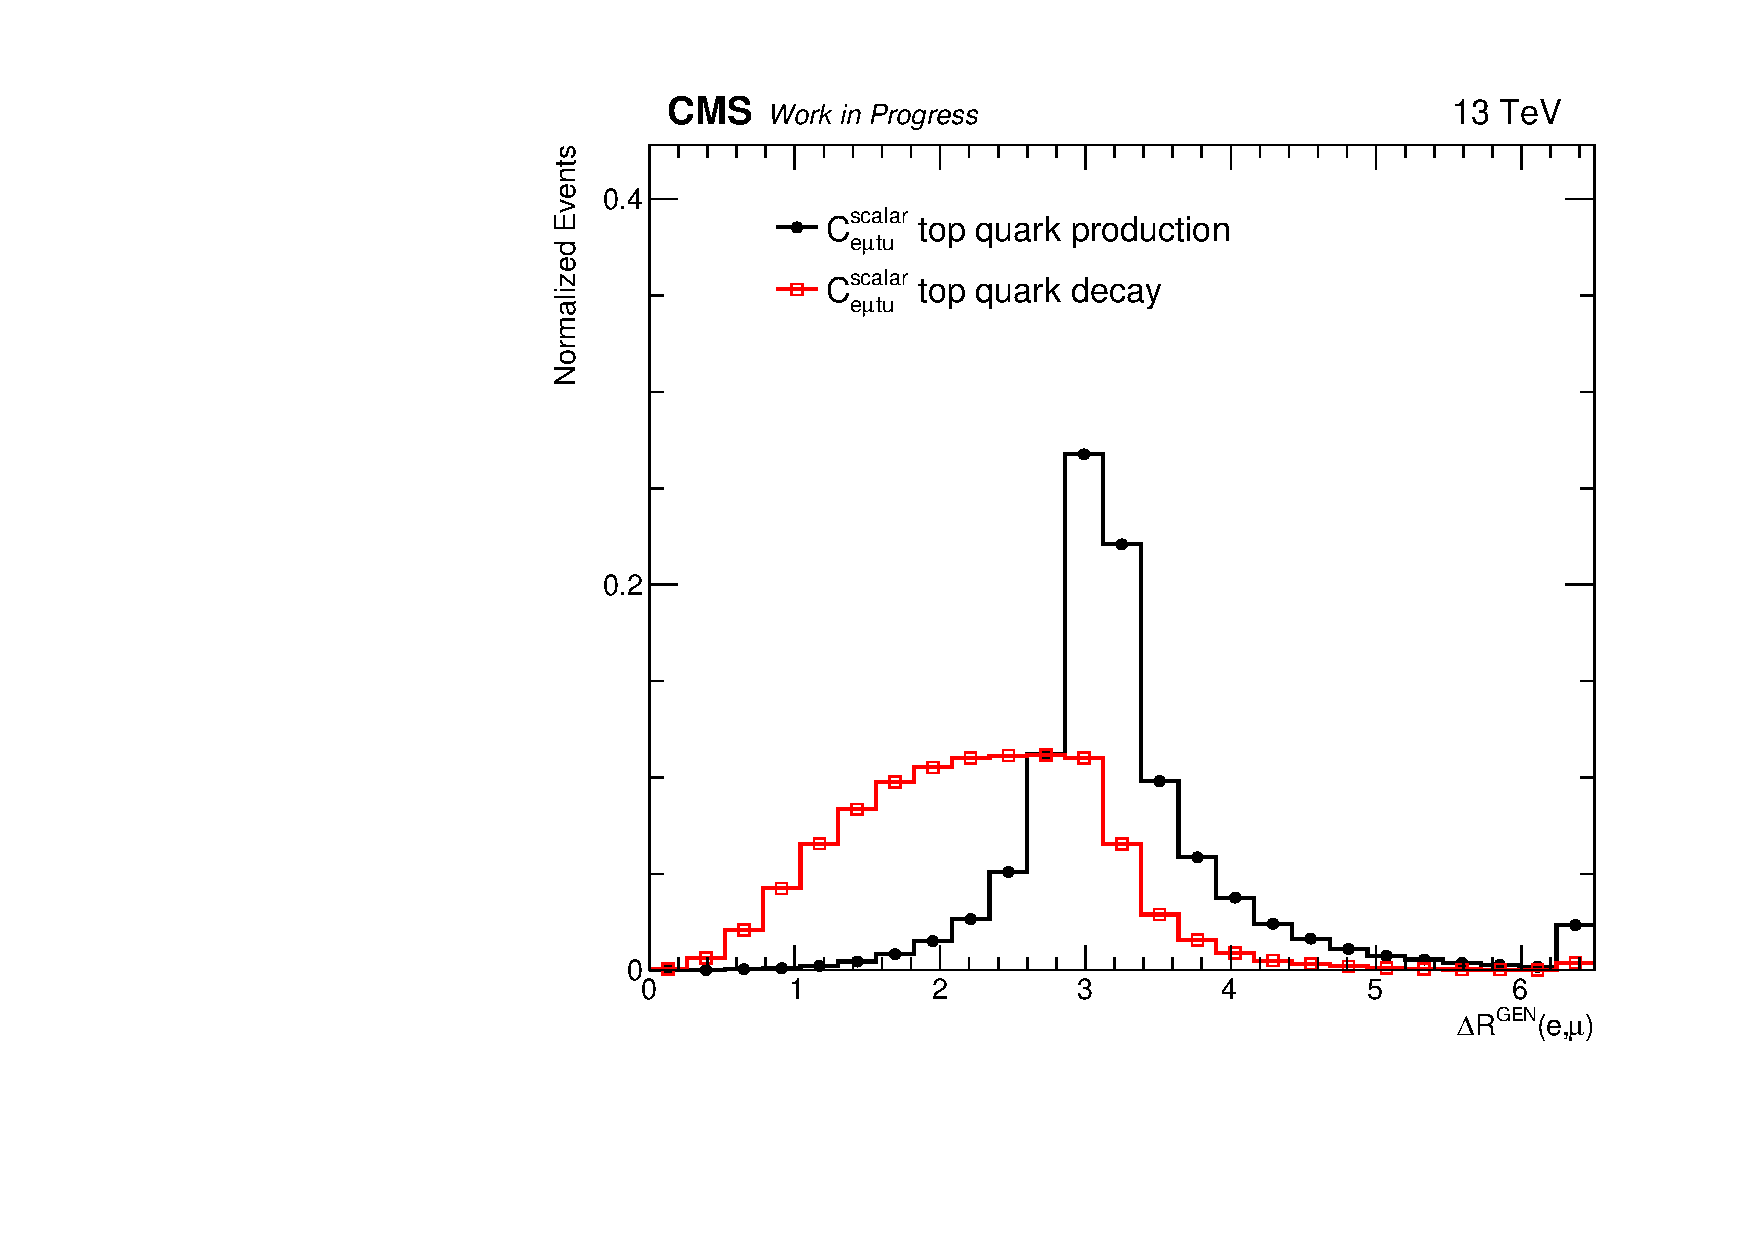
\includegraphics[width=0.33\textwidth]{figures/Part4/Signal/llDr_emu}&
 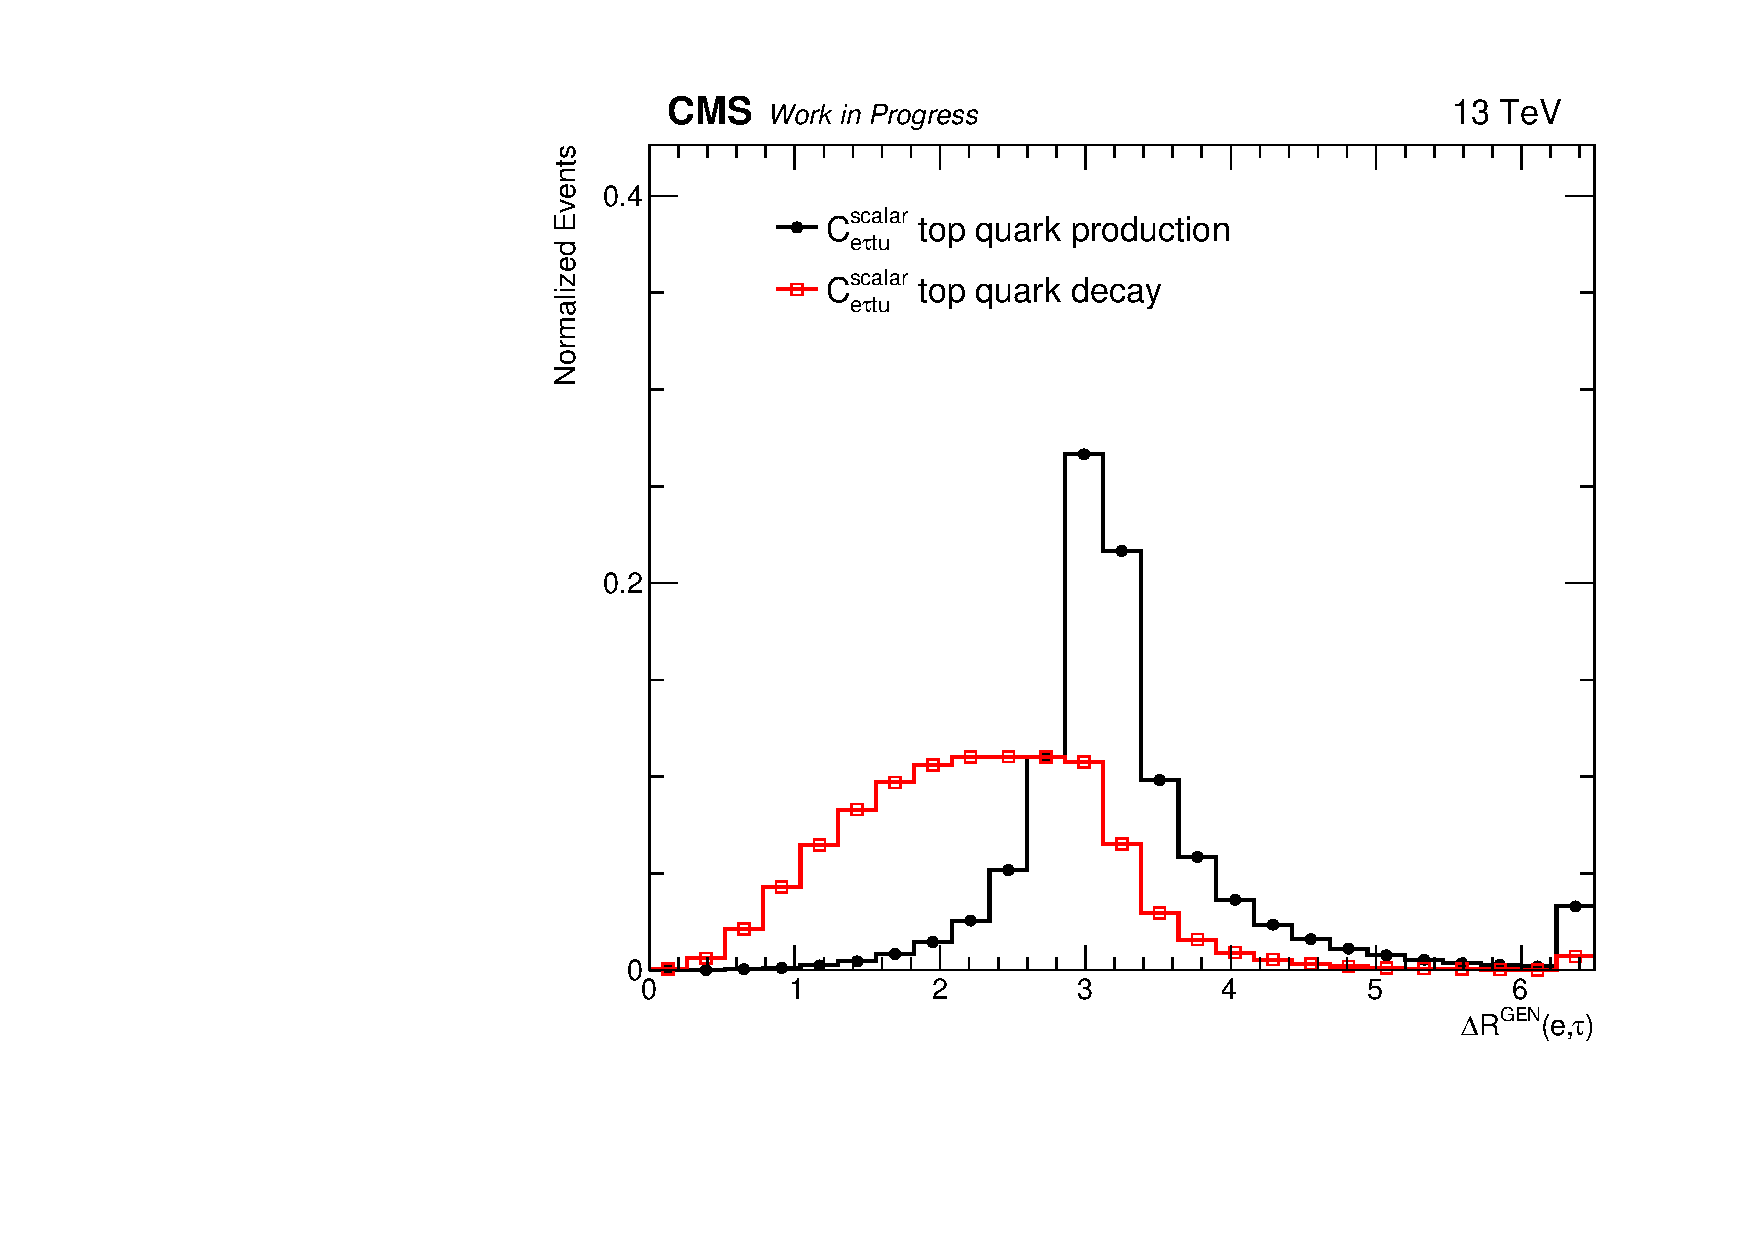
\includegraphics[width=0.33\textwidth]{figures/Part4/Signal/llDr_etau}&
 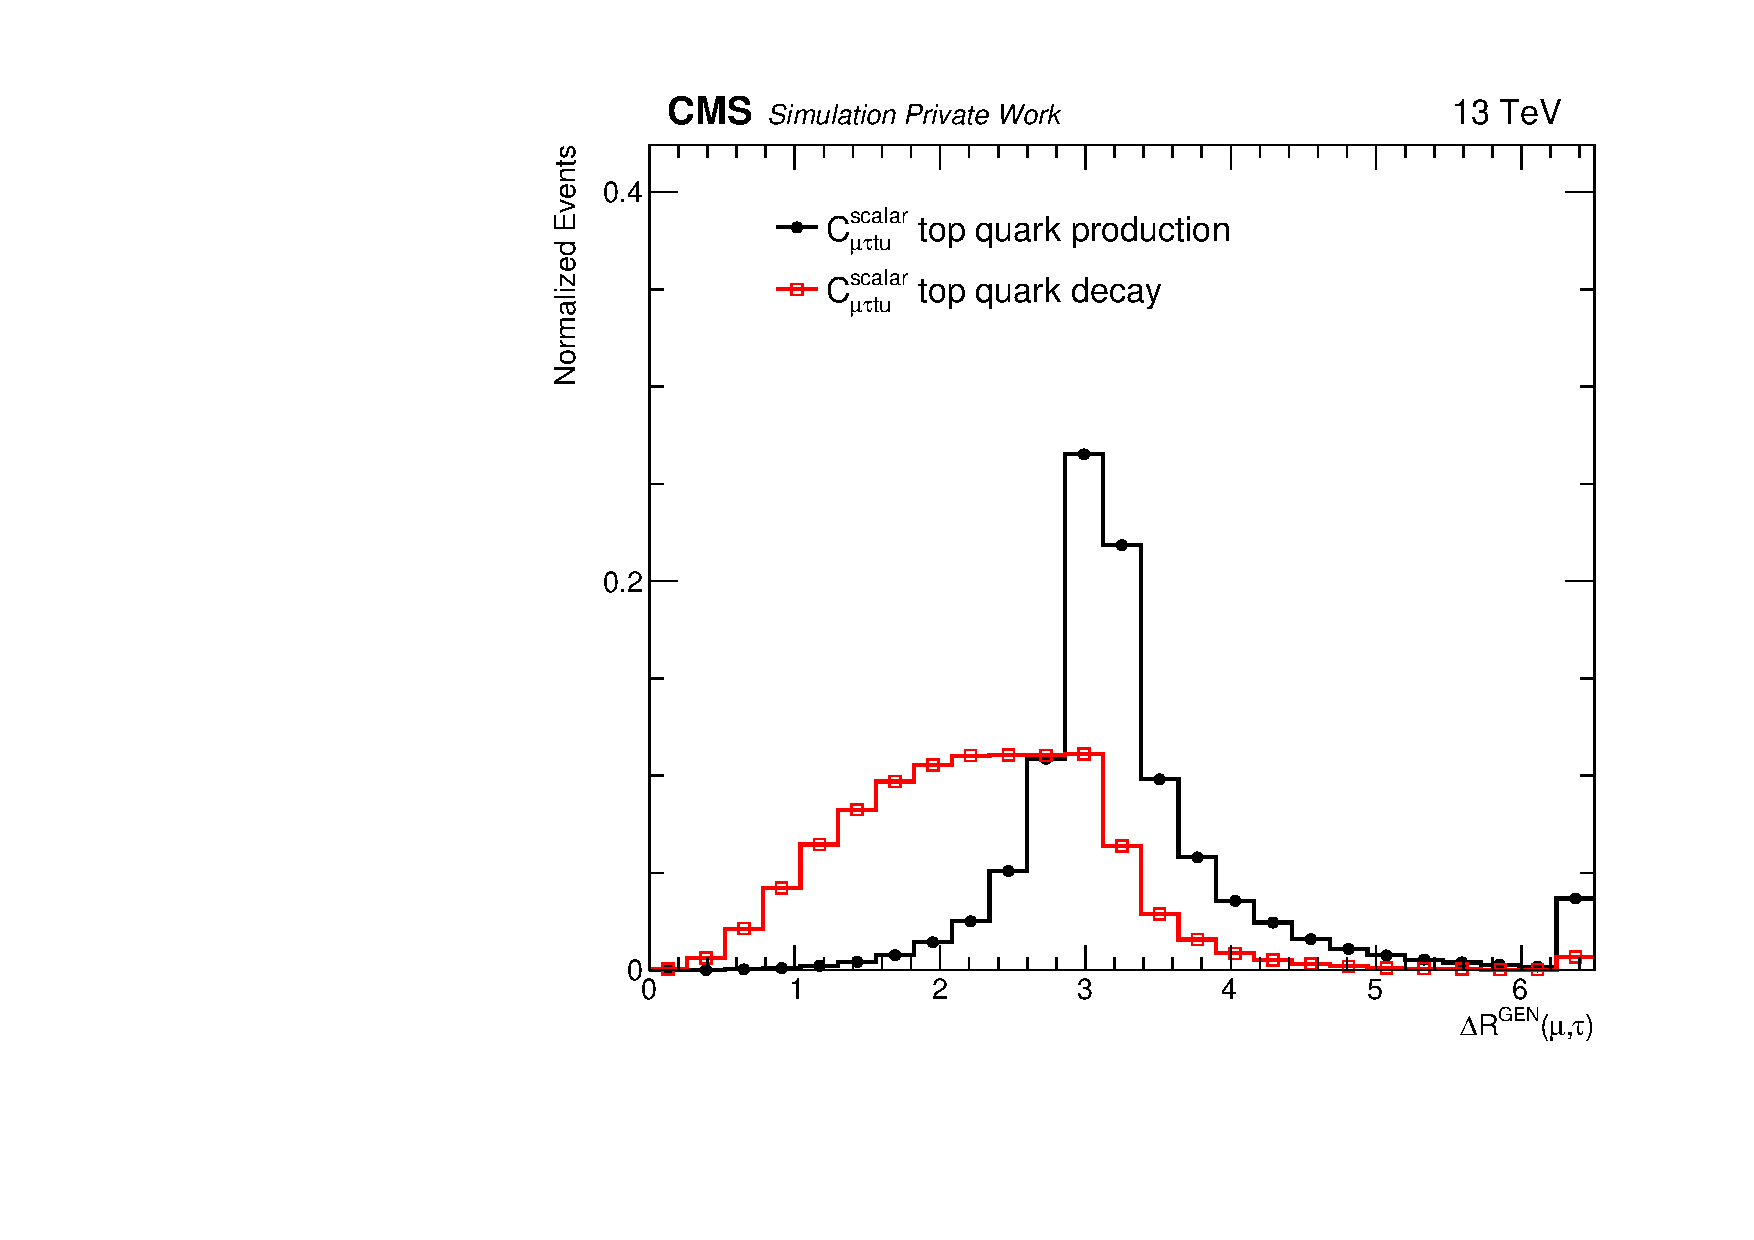
\includegraphics[width=0.33\textwidth]{figures/Part4/Signal/llDr_mutau}\\
 \end{tabular}
 \caption{Normalized kinematic distributions of the \ac{CLFV} signal events at the generator level. These events are generated by the scalar-like operator involving an up quark in the \ac{EFT} vertex. Events from the original samples are categorized into the e$\upmu$ (left), e$\uptau$ (middle), and $\upmu\uptau$ (right) modes. Distributions of the LFV dilepton mass and the opening angle between the two LFV leptons are shown in the top row and the bottom row, respectively. The top quark decay signals are shown in a red line with an open square while the top quark production signals are shown in a black line with a closed circle.}
 \label{fig:SigGen}
 \end{center}
 \end{figure}
\chapter{Object Selection}
\label{chap:Obj}

Similar to the analysis documented in the \autoref{Part3}, the high lepton multiplicity requirement removes the vast majority of the $\ttbar$ and \ac{DY} events produced in the collisions. However, these processes, especially \ac{DY}, still enter and dominate the event selection due to their sheer volumes. In general, $\ttbar$ or \ac{DY} events do not promptly produce three genuine leptons (including hadronic taus), and they can only enter a three-lepton selection if at least one of the light lepton is \emph{nonprompt}, as defined in \autoref{chap:Nonprompt}. Alternatively, jets might also be misidentified as hadronic taus at the reconstruction level, contributing to the so-called ``\emph{fake} tau background''. One example is the \ac{DY}+jets events, where the two \ac{OSSF} light leptons are correctly identified but a jet is misidentified as a hadronic tau. Stringent selection criteria are applied to lepton candidates in order to suppress these backgrounds, which are discussed in \autoref{sec:EandM} and \autoref{sec:Taus}. Additionally, selection criteria on jets and \ac{MET} are discussed in \autoref{sec:JME}.
%%%%%%%%%%%%%%%%%%%%%%%%%%%%%%%%%%%%%%%%%%%%%%%%%%
%%%%%%%%%%%%%%%%%%%%%%%%%%%%%%%%%%%%%%%%%%%%%%%%%%

\section{Electrons and Muons}
\label{sec:EandM}

An updated version of the \TOP\cite{CMS:2023ftu} is used to select \emph{prompt} leptons. The same set of features used in the previous version is also used in this new version even though the training set in this new version is constructed solely from simulated $\ttbar$ events, as opposed to from $\ttbar$, $\ttbar W$, $\ttbar Z$, and tZq. The previous version of the \TOP was originally designed for a multi-lepton analysis like tZq, which is why samples other than $\ttbar$ are included in the training. For this analysis with two leptons (excluding hadronic tau), the new version of the \TOP is better suited. One notable upgrade of this new version is the switch from TMVA \cite{TMVA:2007ngy} to \textsc{XGBoost} \cite{Chen:2016:XST:2939672.2939785} in its \ac{BDT} implementation. This improves the signal efficiency by a few percentage points while keeping the same background efficiency. 

Both electron and muon candidates are required to have a minimum \TOP score of 0.64, corresponding to roughly the same background efficiency (1\%) that is chosen for the previous analysis. However, this working point corresponds to a signal efficiency of 92\%, which is 2\% higher than the previous implementation.

On top of the \TOP requirement, a set of selection criteria are added to select electron and muon candidates, which are largely derived from the existing strategy described in \autoref{sec:Leptons}. The minimum $\pt$ requirement is lowered from 38 GeV to 30 GeV for the leading lepton when compared to the previous analysis. This change helps improve the signal acceptance as this analysis faces even lower statistics. The $\pt$ threshold on the sub-leading lepton is kept at 20 GeV. The requirements on $\eta$, $d_{\textsf{xy}}$, $d_{\textsf{z}}$, and SIP$_3$ are kept the same as they come from the same pre-selection requirements used in the \ac{BDT} training. 

The same ``mini isolation'' variable $I^{\textsf{rel}}_{\textsf{mini}}$ defined in Equation~\ref{eq:mini} is used to create isolated lepton candidates, even though the threshold is loosened from 0.12 to 0.4. Similar to the lowering of of the $\pt$ on the leading lepton, this change helps improve the signal acceptance.

Only lepton candidates that pass all the requirements stated above are considered in this analysis. They are referred to as ``\emph{tight}'' leptons, which does not include hadronic tau.
%%%%%%%%%%%%%%%%%%%%%%%%%%%%%%%%%%%%%%%%%%%%%%%%%%
%%%%%%%%%%%%%%%%%%%%%%%%%%%%%%%%%%%%%%%%%%%%%%%%%%

\section{Hadronic Taus}
\label{sec:Taus}

A \ac{NN}-based algorithm called ``\textsc{DeepTau}''~\cite{CMS:2022prd} is used to simultaneously discriminate
against jets, electrons, and muons. The core feature of this algorithm is the use of convolutional layers to exploit the translational invariance of the input variables. A combination of lower-level and high-level variables are used as input features to the \ac{NN}. The lower-level variables are derived from individual particles reconstructed by the \ac{PF} algorithm while the high-level variables are mostly taken from the previously trained \ac{MVA}~\cite{CMS:2015pac}. Two grids are defined in $\eta-\phi$ plane to encode the positions as well as other low-level inputs from \ac{PF} candidates. The outer grid and the inner grid consist of 21$\times$21 cells and 11$\times$11 cells, respectively. The total number of input variables is 105703, which consists of 188 low-level variables per grid cell and 47 high-level variables.

When compared to the discriminators from existing algorithms~\cite{CMS:2018jrd,CMS:2015pac}, the discriminators against jets and electrons from the \textsc{DeepTau} algorithm provide a 10-30\% improvement in signal efficiency while maintaining the same background efficiency. The discriminator against muons from the \textsc{DeepTau} algorithm provides a factor of 3-10 larger background rejection while maintaining the signal efficiency at a very high level (99.1-99.4\%).

Tau candidates are required to simultaneously pass ``VLoose'', ``Tight'', and ``Tight'' working points of the discriminators against electrons, muons, and jets, respectively. These working points correspond to over 99\% signal efficiency for discriminators against electrons and muons, and 60\% for the discriminator against jets. The working point chosen for the discriminator against jets is a lot tighter as the vast majority of \emph{fake} taus in this analysis originate from jets.

In addition to the \textsc{DeepTau} working points, a set of selection criteria is applied to tau candidates, which is mostly derived from the pre-selection requirements of the \textsc{DeepTau} algorithm. Tau candidates are required to have a minimum $pt$ of 20 GeV with $|\eta|~<$ 2.3. Similar to the requirements on electron and muon candidates, $|d_{\textsf{xy}}|$ and $|d_{\textsf{z}}|$ of tau candidates are required to be smaller than 0.05 and 0.1, respectively. Tau candidates reconstructed from decay modes with missing charged hadrons are excluded.

To enter the event selection of this analysis, tau candidates are required to pass all the requirements stated above. Tau candidates that satisfy all the requirements are referred to as ``\emph{tight}'' taus in this analysis.
%%%%%%%%%%%%%%%%%%%%%%%%%%%%%%%%%%%%%%%%%%%%%%%%%%
%%%%%%%%%%%%%%%%%%%%%%%%%%%%%%%%%%%%%%%%%%%%%%%%%%

\section{Jets}
\label{sec:JME}

Strategy to select jet candidates described in \autoref{sec:Jets} are largely kept intact. The only notable change is the lowering of the $\pt$ threshold of jets from 30 GeV to 25 GeV. The \DeepJ algorithm~\cite{Bols:2020bkb} described in \autoref{sec:Btag} is also used to tag jets that originate from b quark in this analysis. The ``Loose'' working point is chosen to tag b jet candidates, which corresponds to roughly 10\% improvement in signal efficiency when compared to the ``Medium'' working point used by the previous analysis.
\chapter{Event Selection}
\label{chap:Evt}



%%%%%%%%%%%%%%%%%%%%%%%%%%%%%%%%%%%%%%%%%%%%%%%%%%
%%%%%%%%%%%%%%%%%%%%%%%%%%%%%%%%%%%%%%%%%%%%%%%%%%
\section{Event Categorization}
\label{sec:Cat}

\begin{figure}[tbh!]
 \begin{center}
 \begin{tabular}{c}
 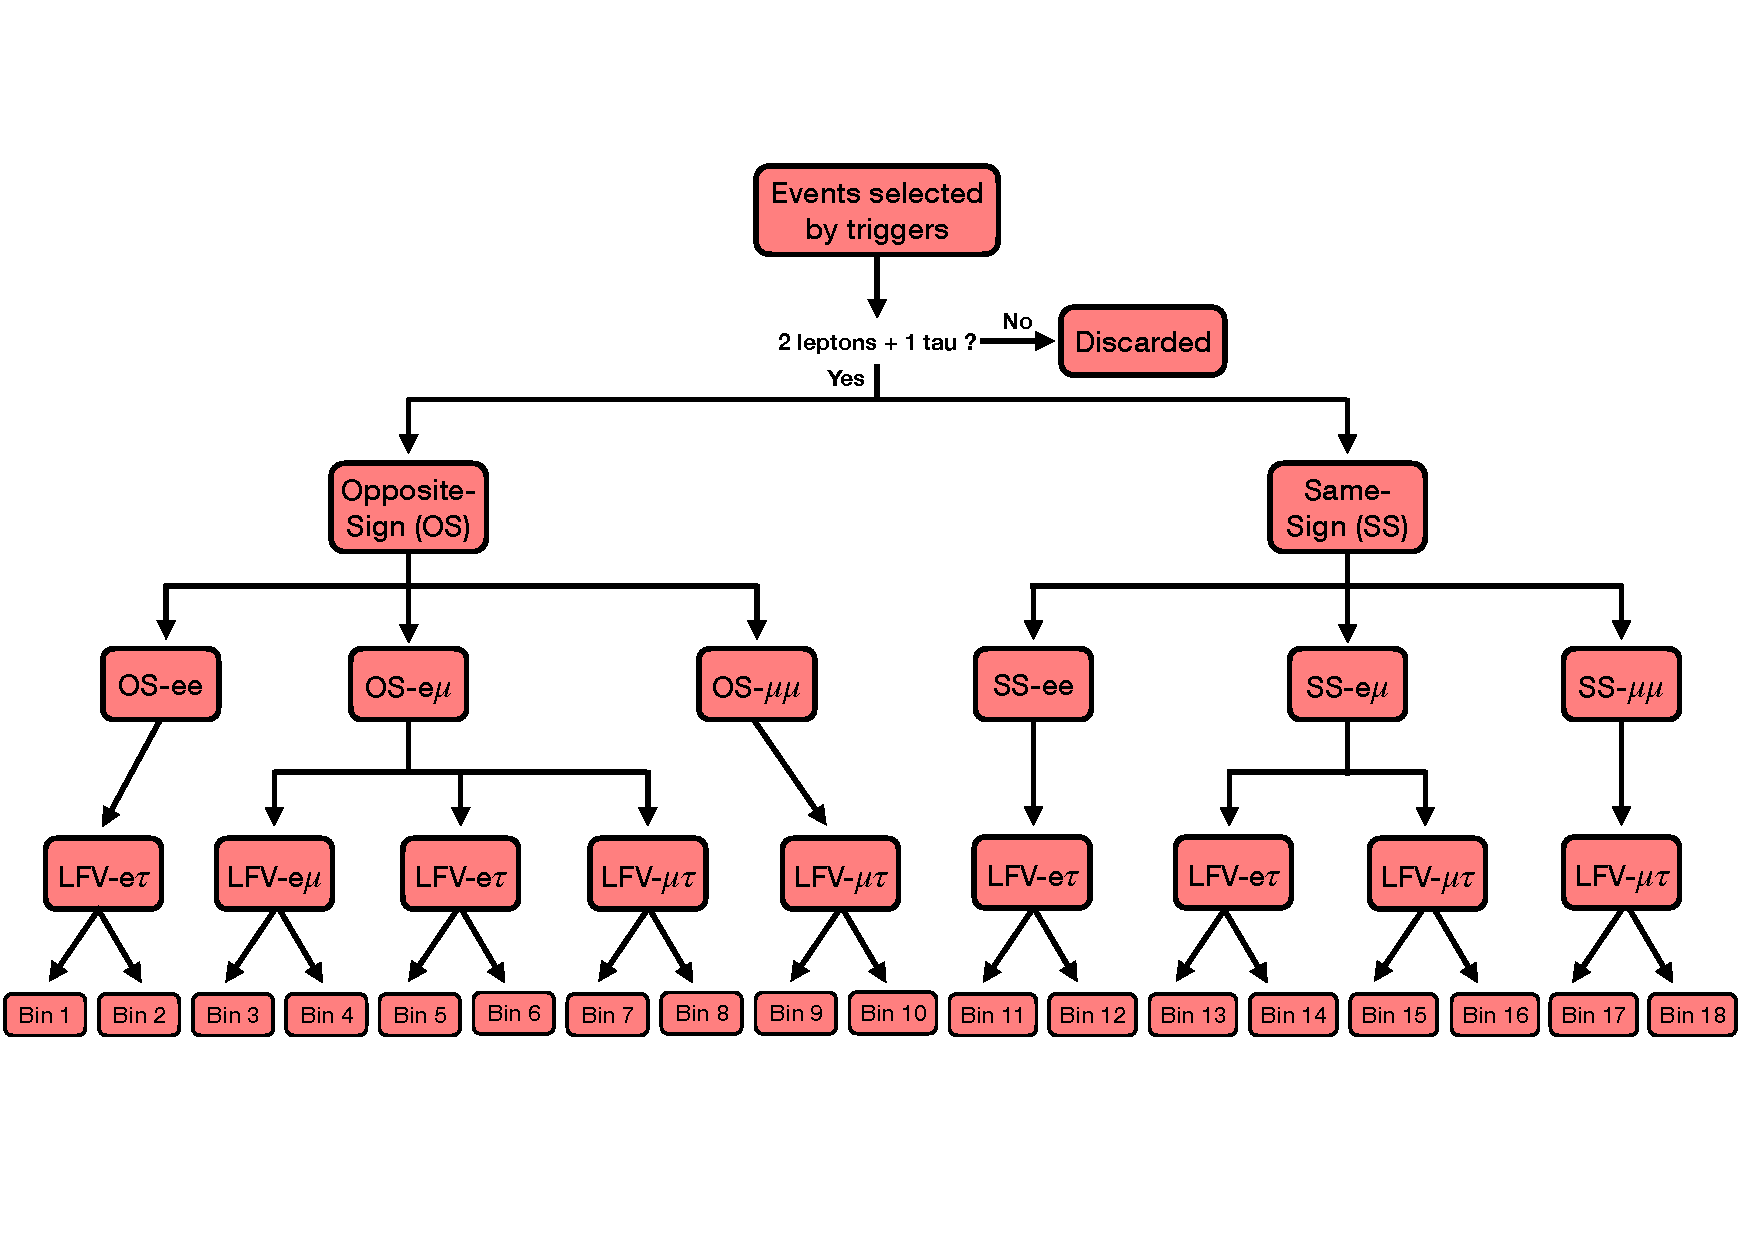
\includegraphics[width=\textwidth]{figures/Part4/Evt/SRFlowChart}
 \end{tabular}
 \caption{XX}
 \label{fig:EvtCat}
 \end{center}
 \end{figure}
%%%%%%%%%%%%%%%%%%%%%%%%%%%%%%%%%%%%%%%%%%%%%%%%%%
%%%%%%%%%%%%%%%%%%%%%%%%%%%%%%%%%%%%%%%%%%%%%%%%%%

\section{Signal Region}
\label{sec:SRInclusive}

\begin{figure}[tbh!]
 \begin{center}
 \begin{tabular}{c}
 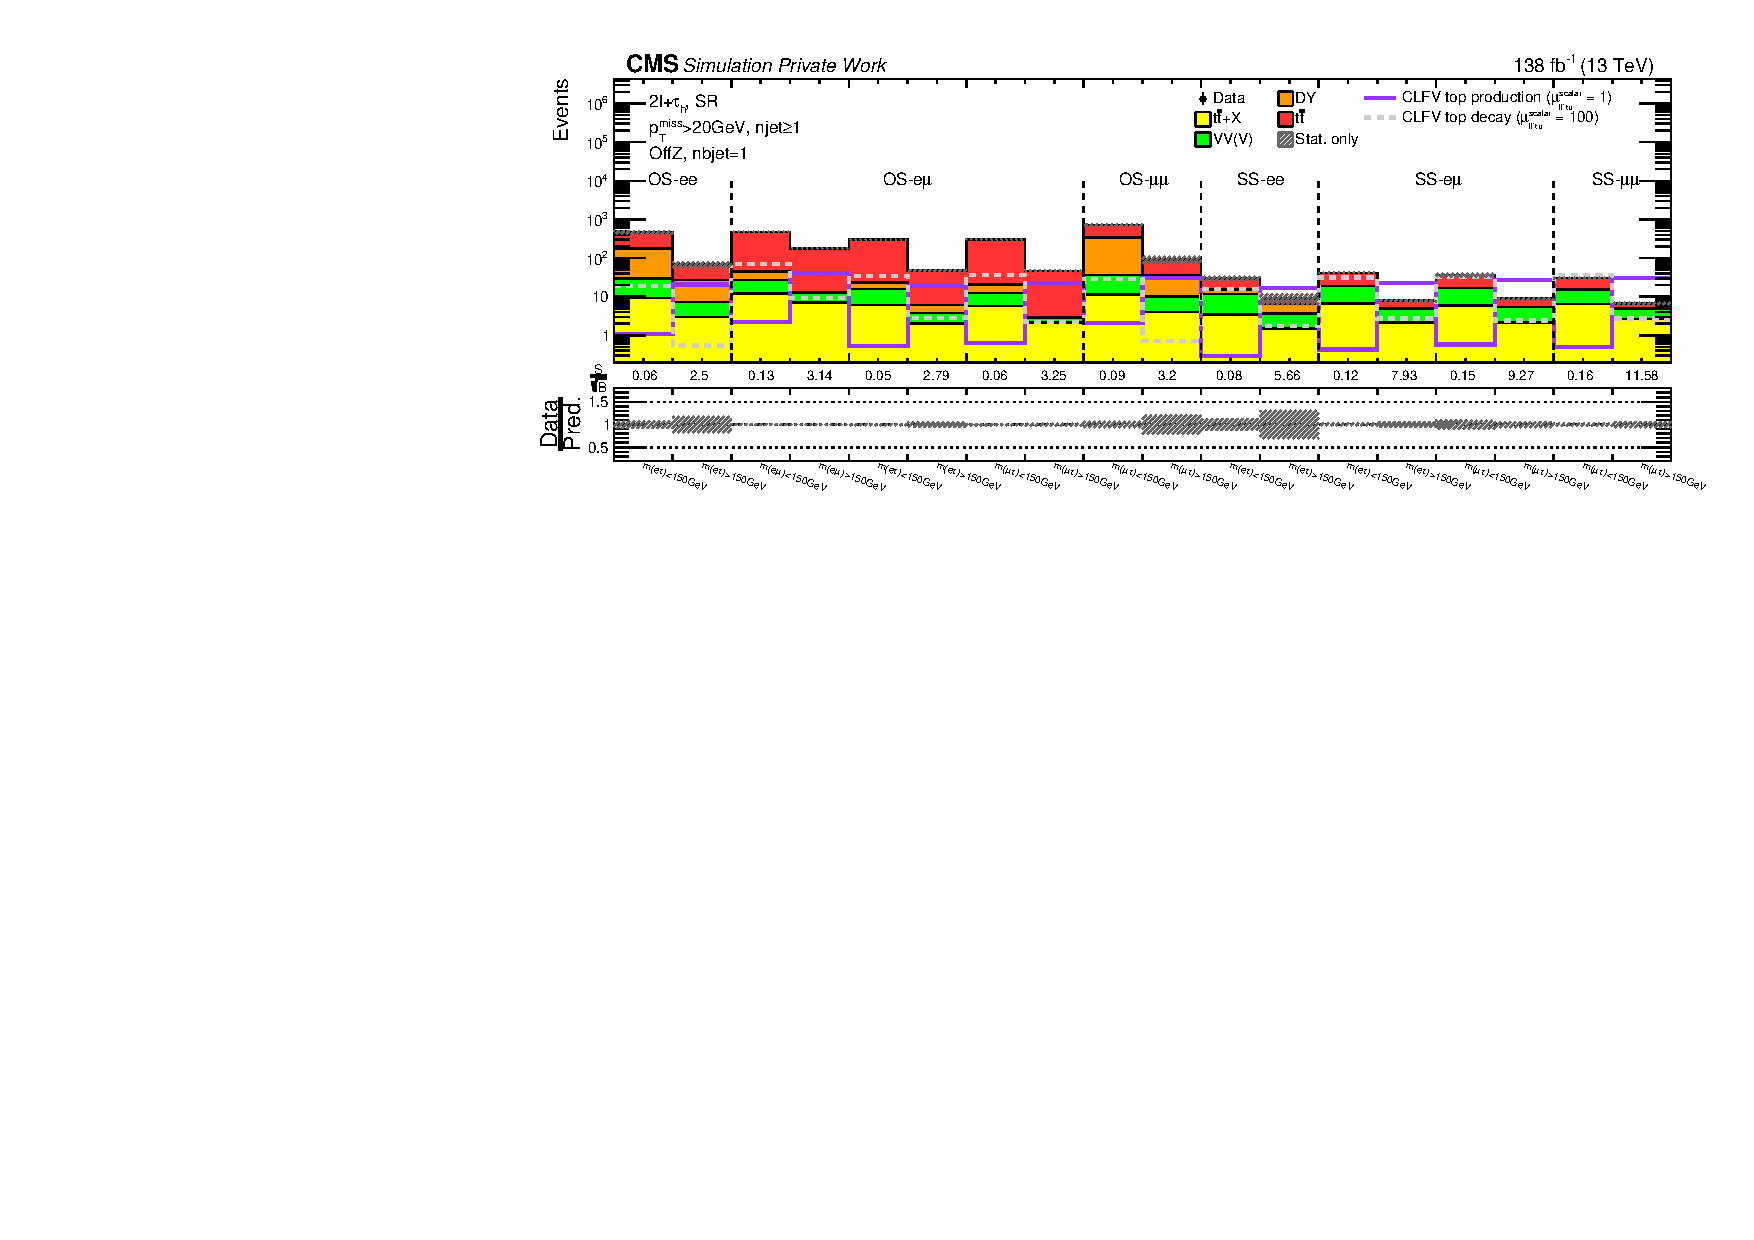
\includegraphics[width=\textwidth]{figures/Part4/Evt/Summary_llOffZMetg20B1}
 \end{tabular}
 \caption{XX}
 \label{fig:Summary}
 \end{center}
 \end{figure}
 
 \begin{figure}[tbh!]
 \begin{center}
 \begin{tabular}{c}
 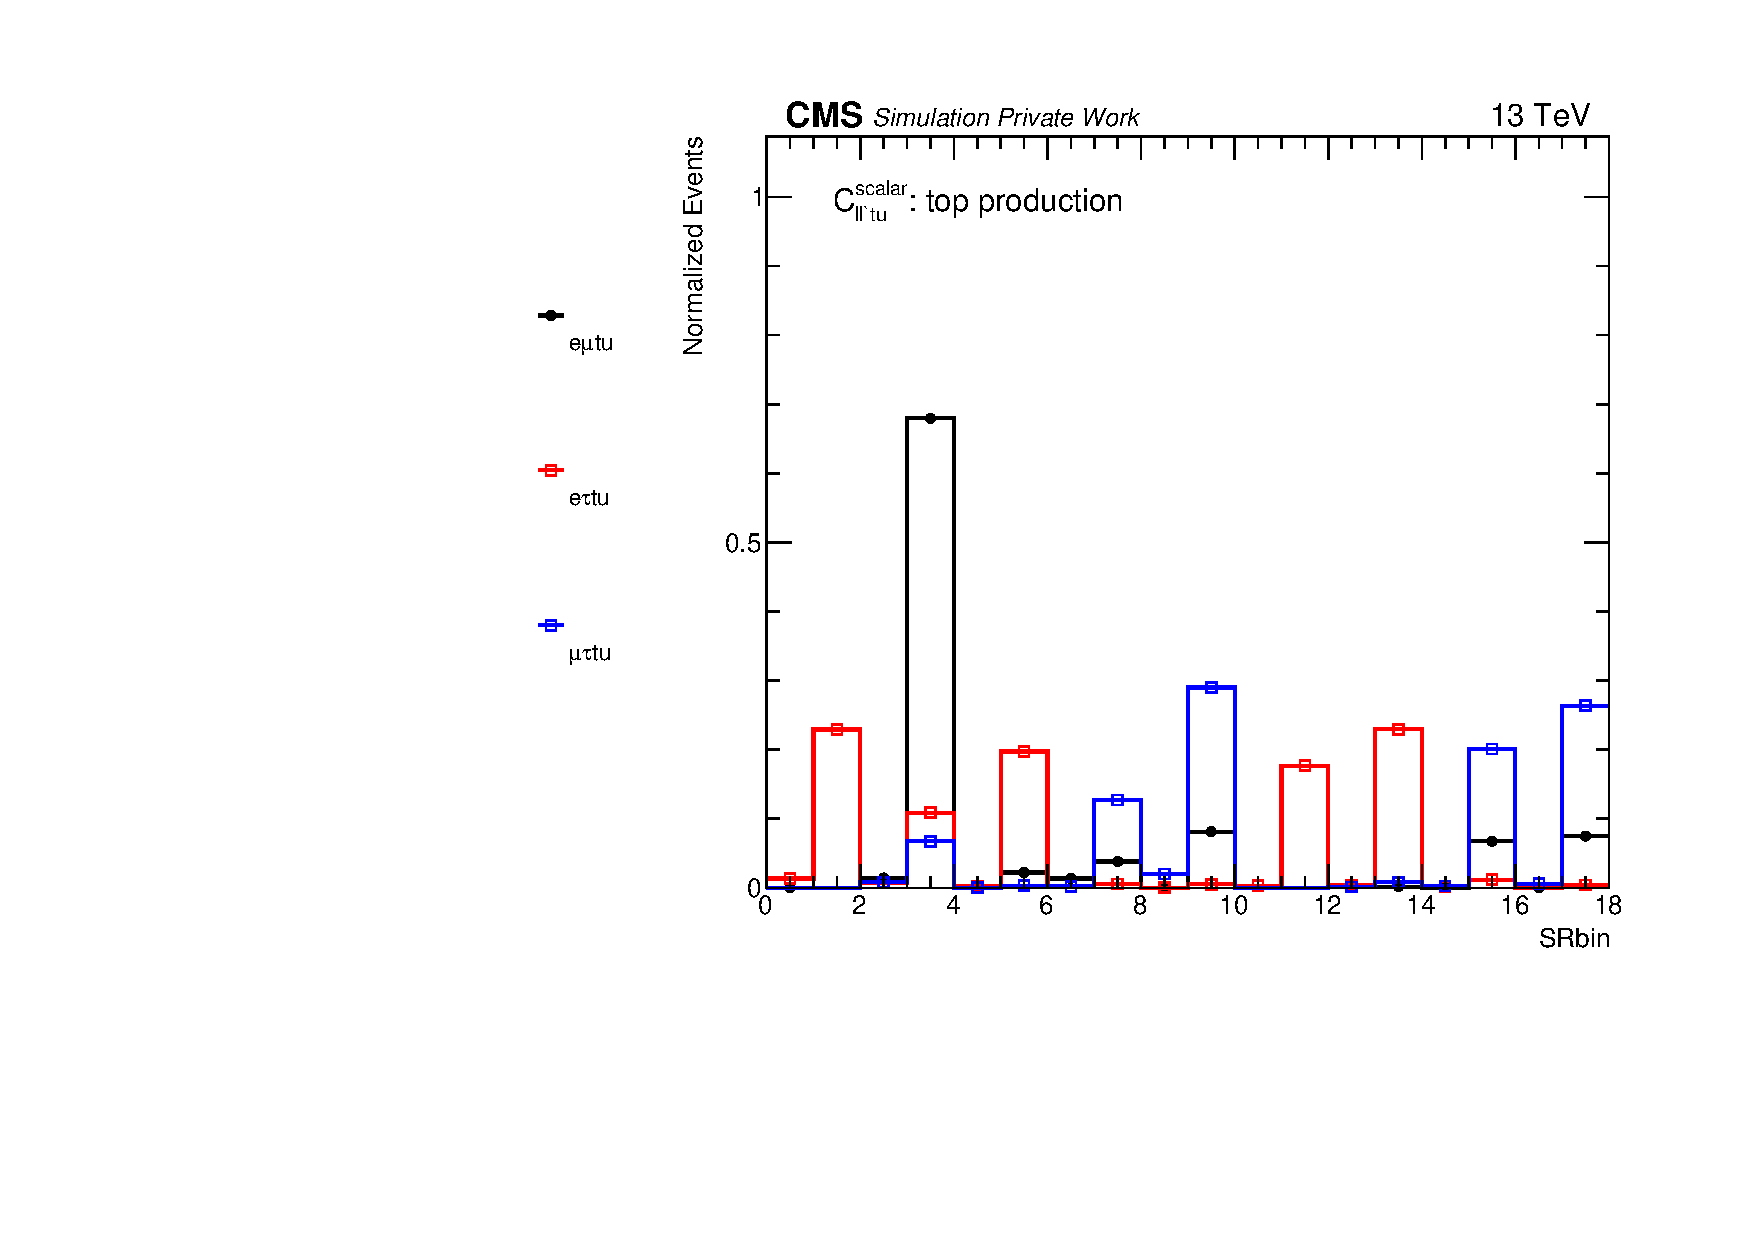
\includegraphics[width=\textwidth]{figures/Part4/Evt/SRbin}
 \end{tabular}
 \caption{XX}
 \label{fig:SRbin}
 \end{center}
 \end{figure}
 
 \begin{figure}[tbh!]
 \begin{center}
 \begin{tabular}{ccc}
 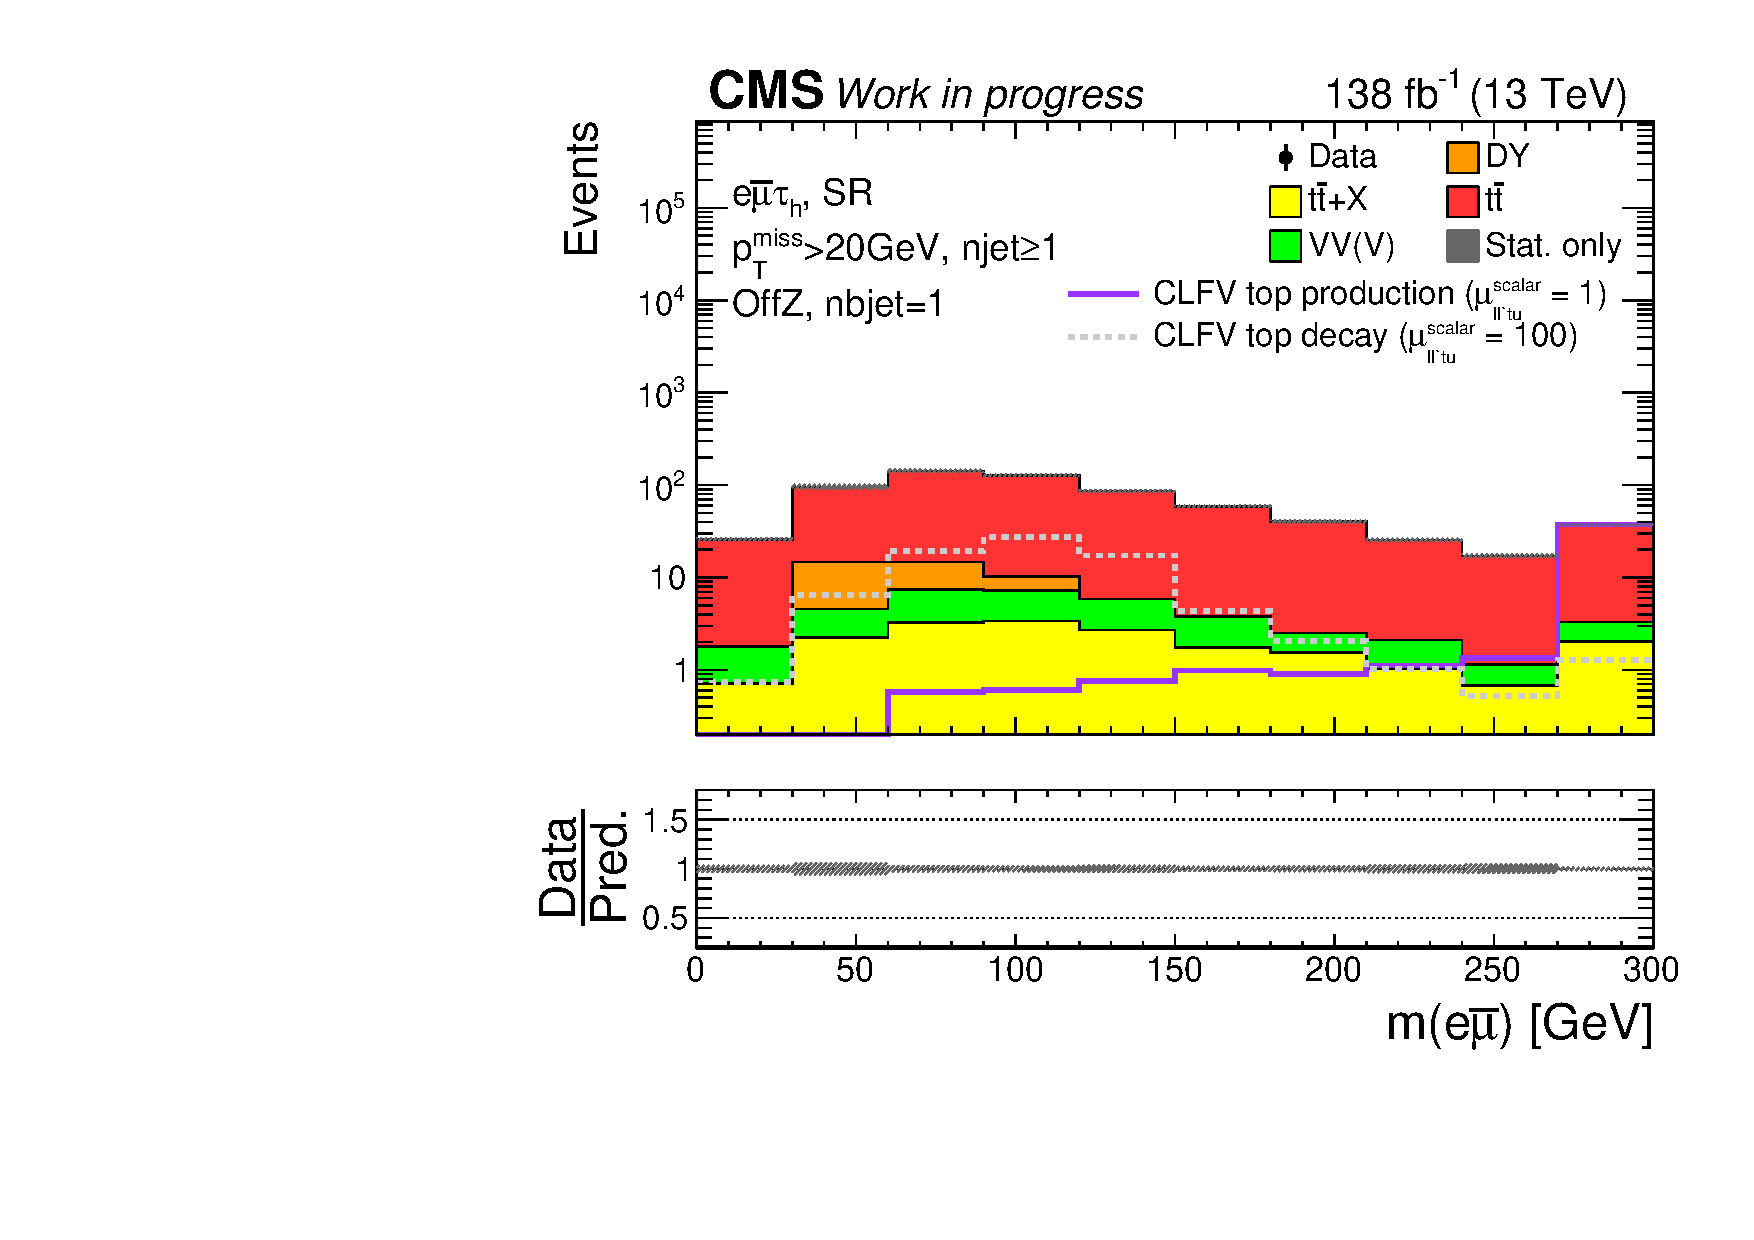
\includegraphics[width=0.33\textwidth]{figures/Part4/Evt/LFVemuM}&
  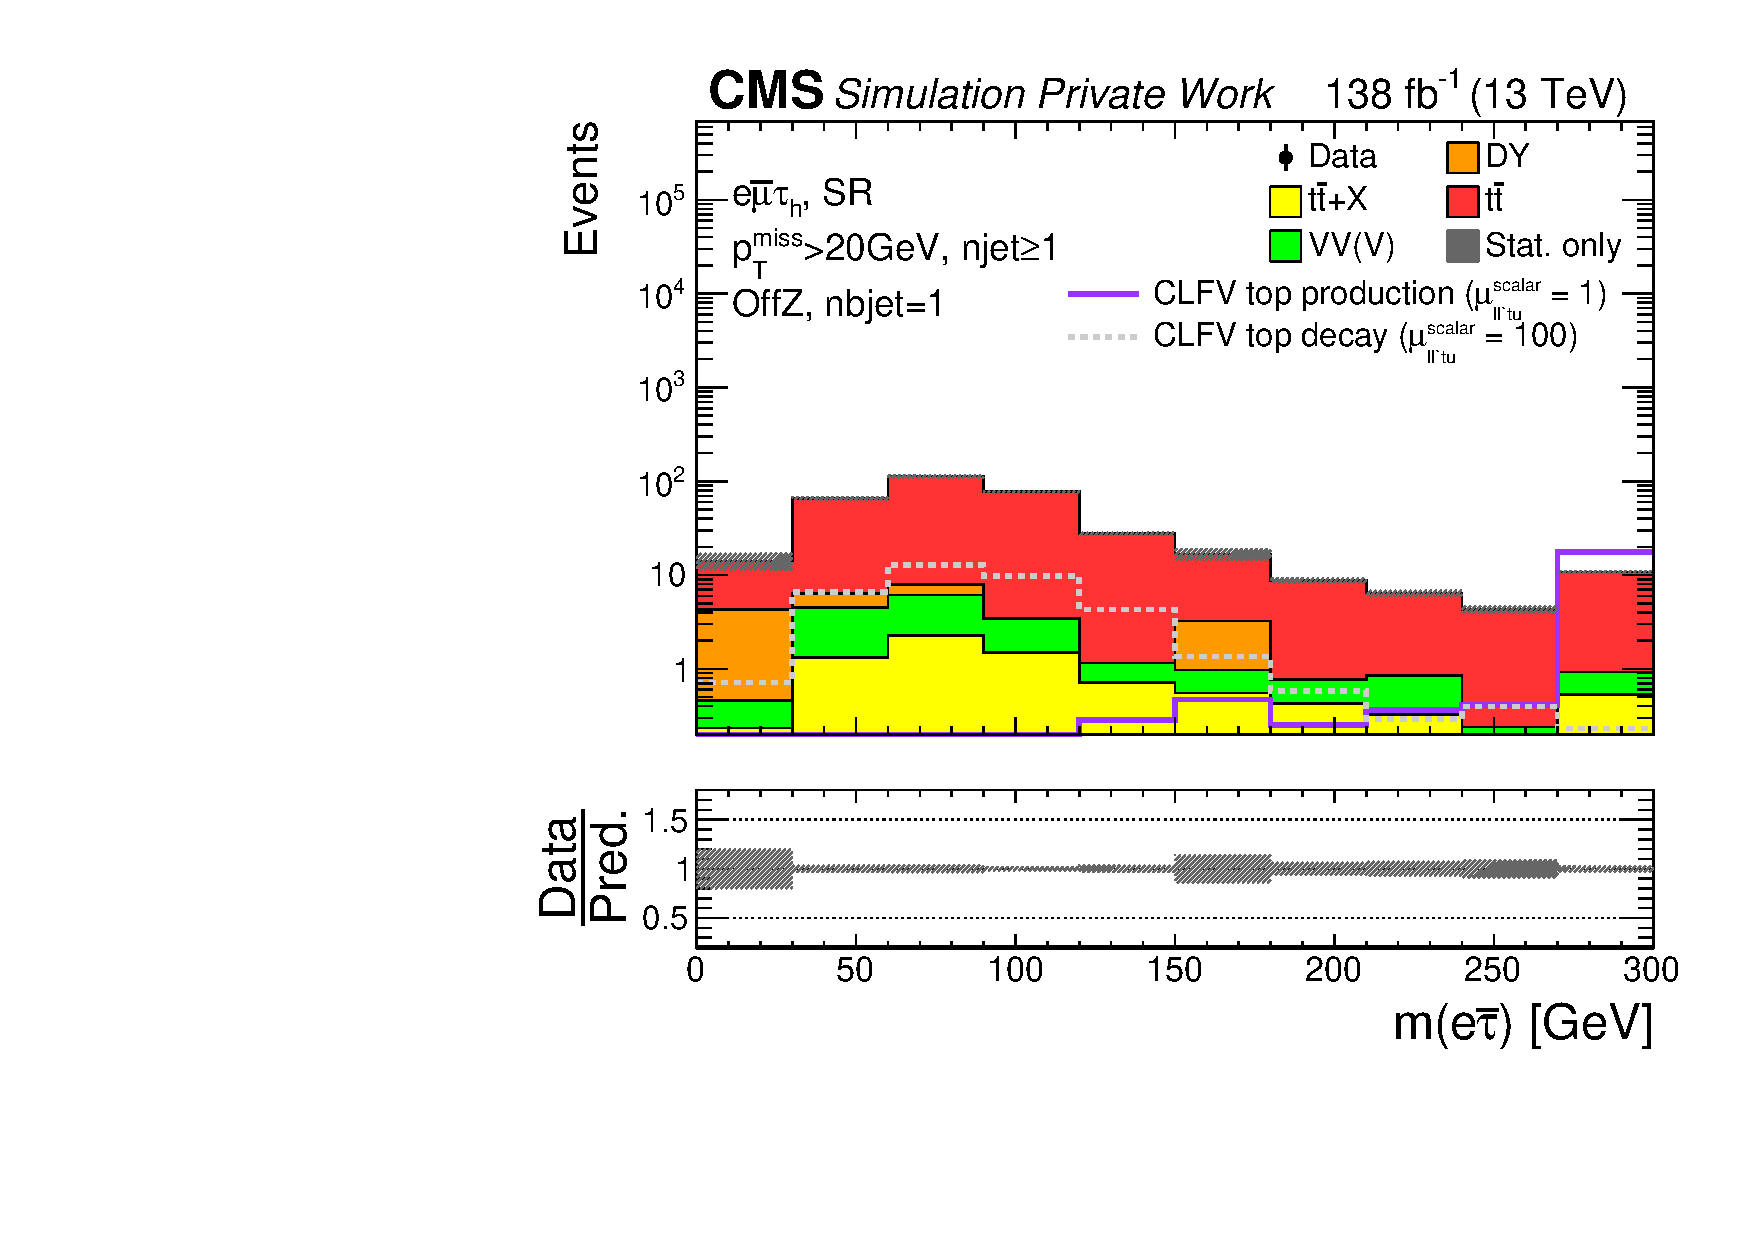
\includegraphics[width=0.33\textwidth]{figures/Part4/Evt/LFVetaM}&
   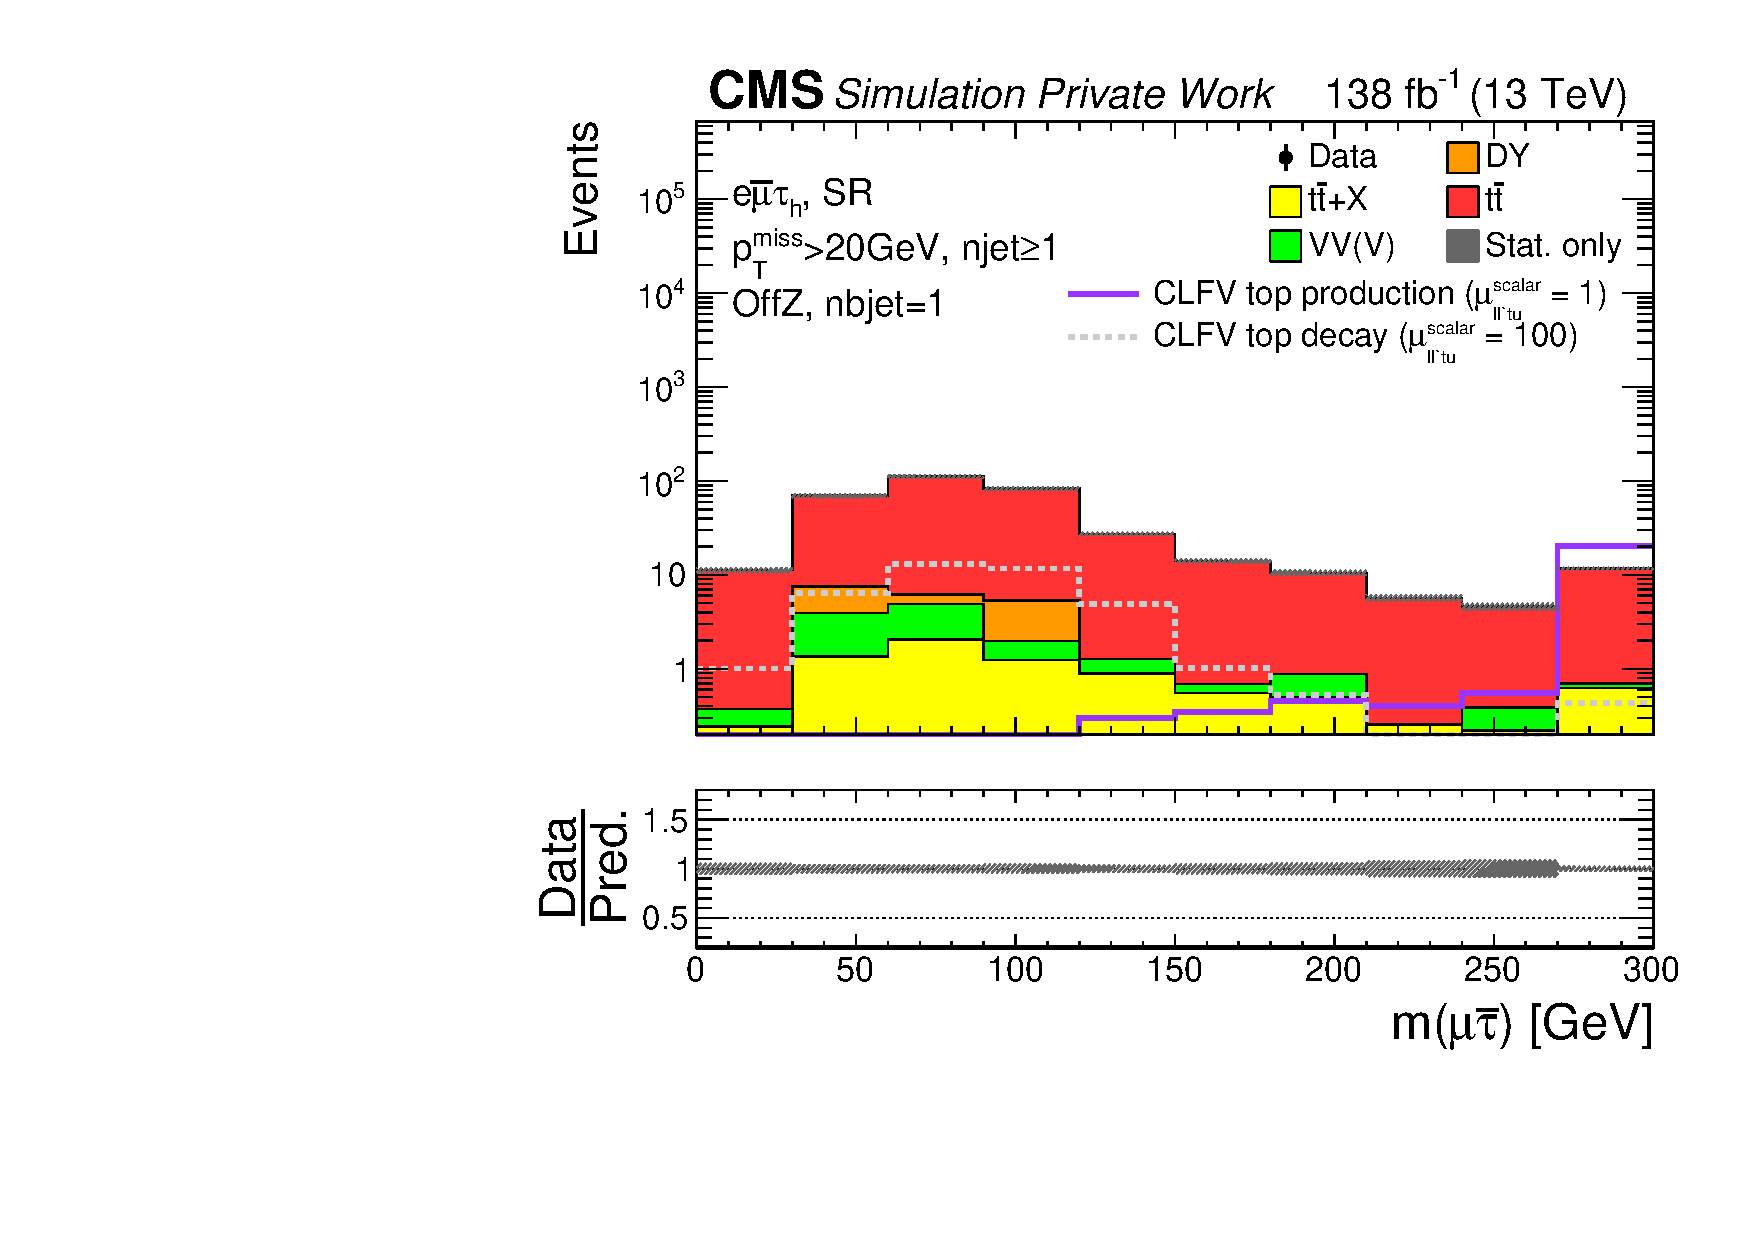
\includegraphics[width=0.33\textwidth]{figures/Part4/Evt/LFVmutaM}\\
 \end{tabular}
 \caption{XX}
 \label{fig:LFVmass}
 \end{center}
 \end{figure}
%%%%%%%%%%%%%%%%%%%%%%%%%%%%%%%%%%%%%%%%%%%%%%%%%%
%%%%%%%%%%%%%%%%%%%%%%%%%%%%%%%%%%%%%%%%%%%%%%%%%%

\section{Drell-Yan Control Region}
\label{sec:DY_CR}

 \begin{figure}[tbh!]
 \begin{center}
 \begin{tabular}{cc}
 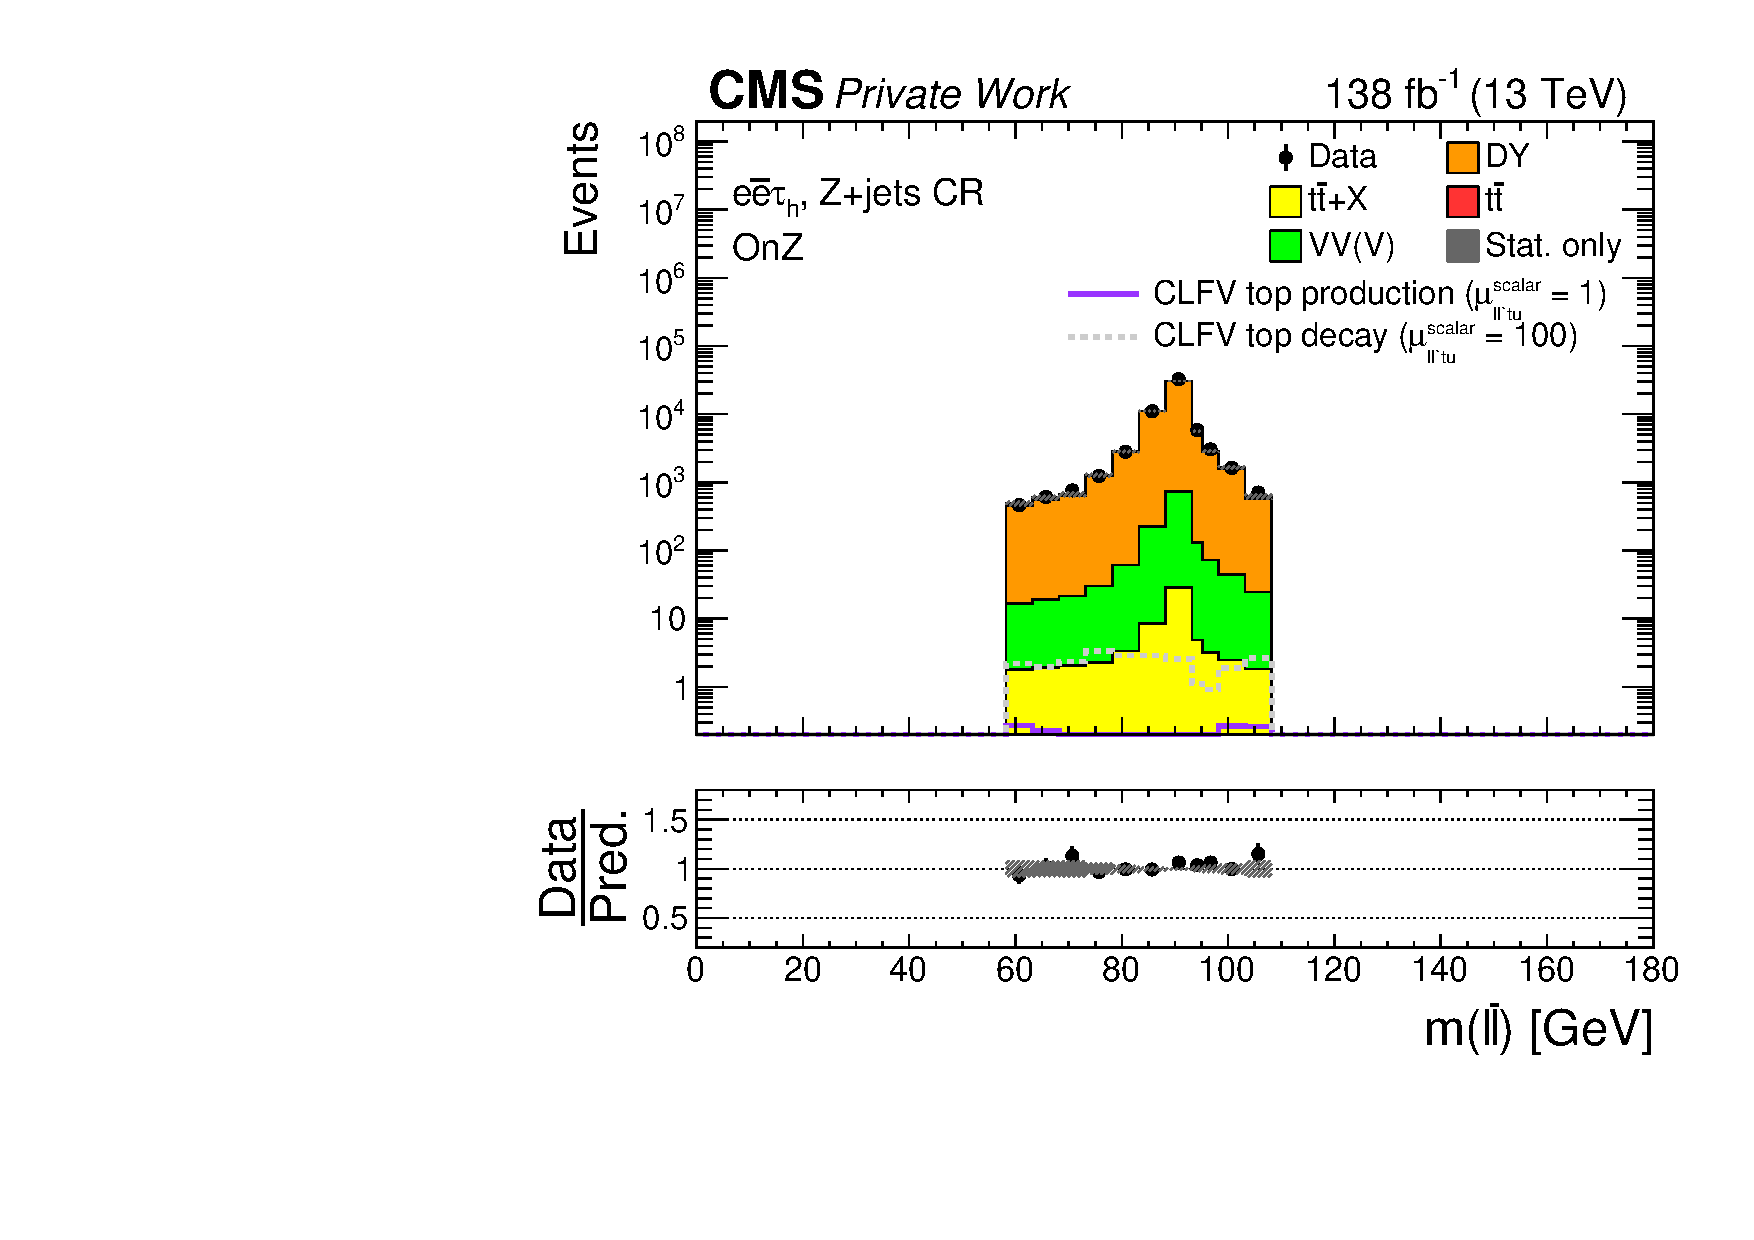
\includegraphics[width=0.48\textwidth]{figures/Part4/Evt/llM_OnZ_ee}&
 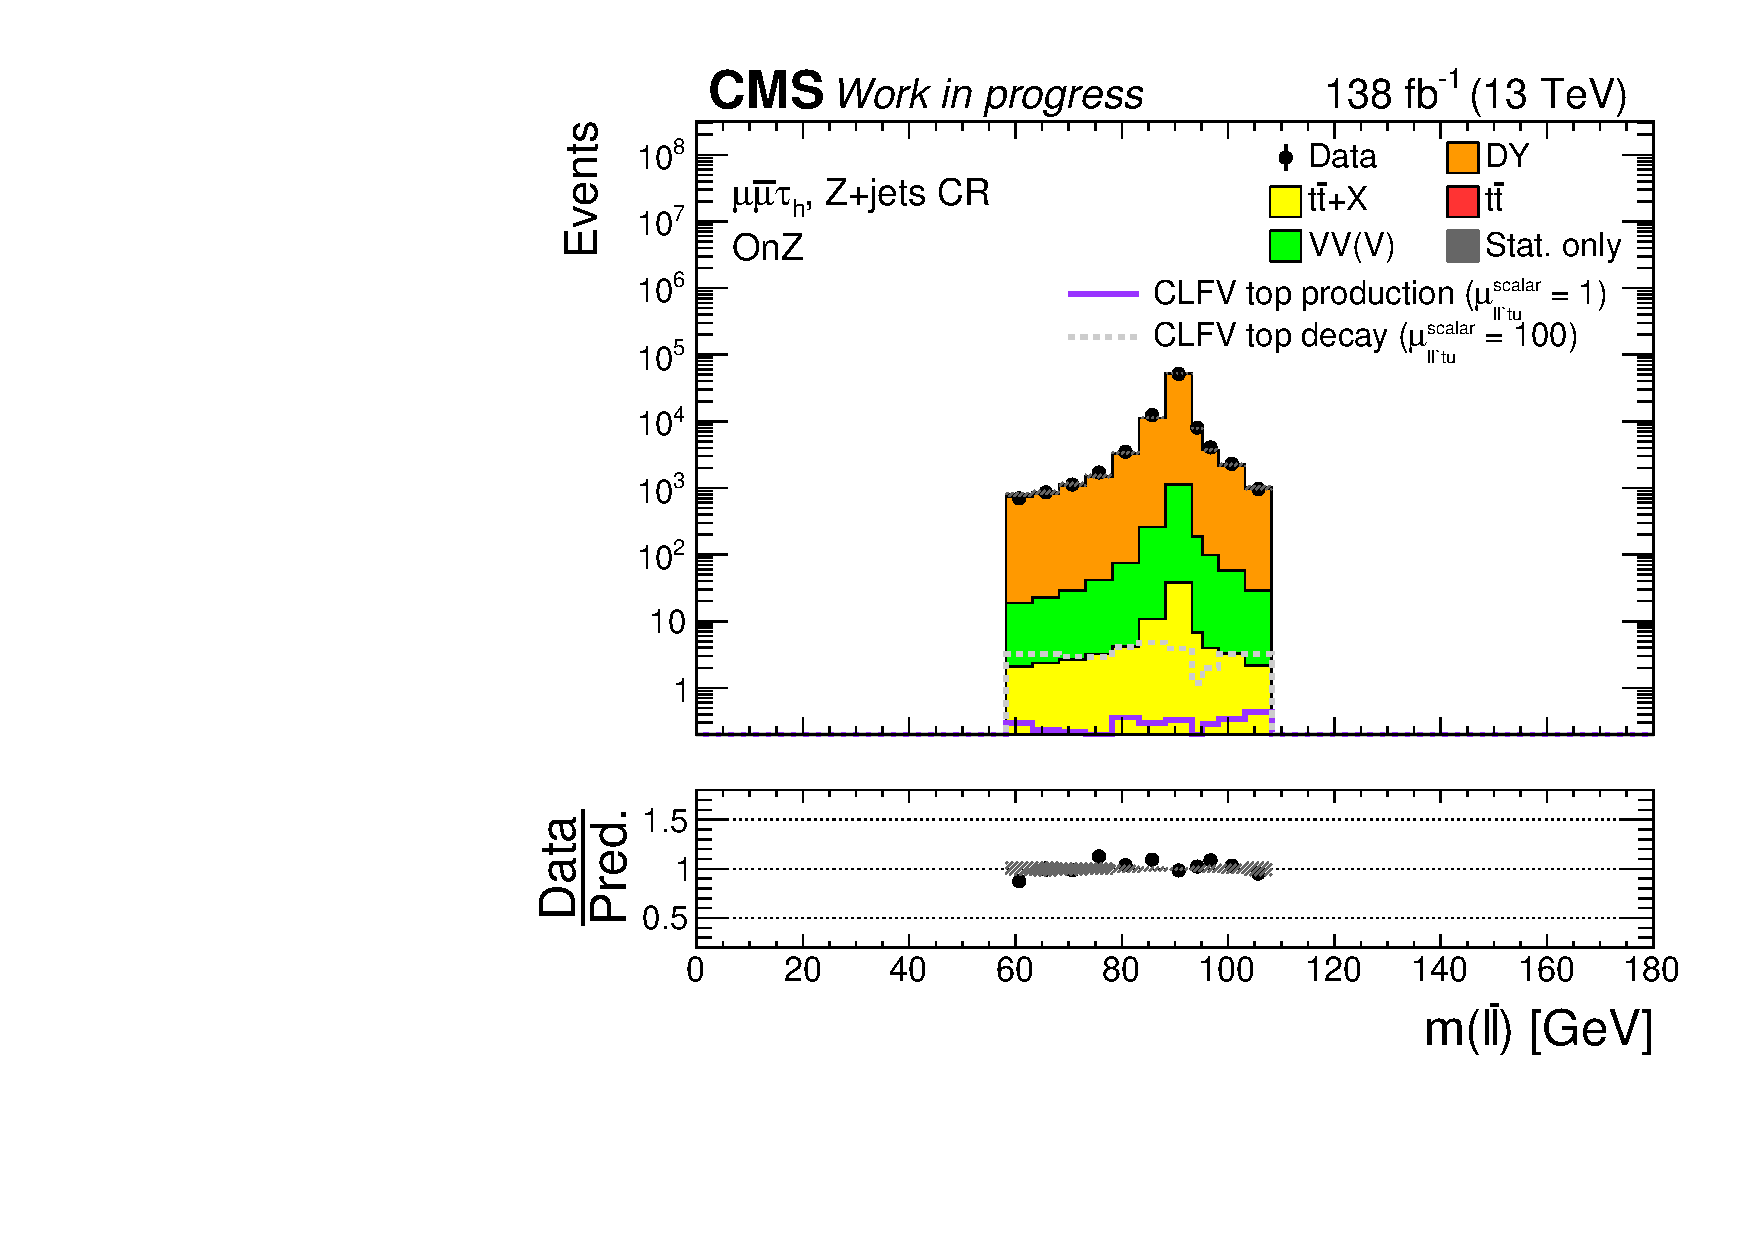
\includegraphics[width=0.48\textwidth]{figures/Part4/Evt/llM_OnZ_mumu}\\
  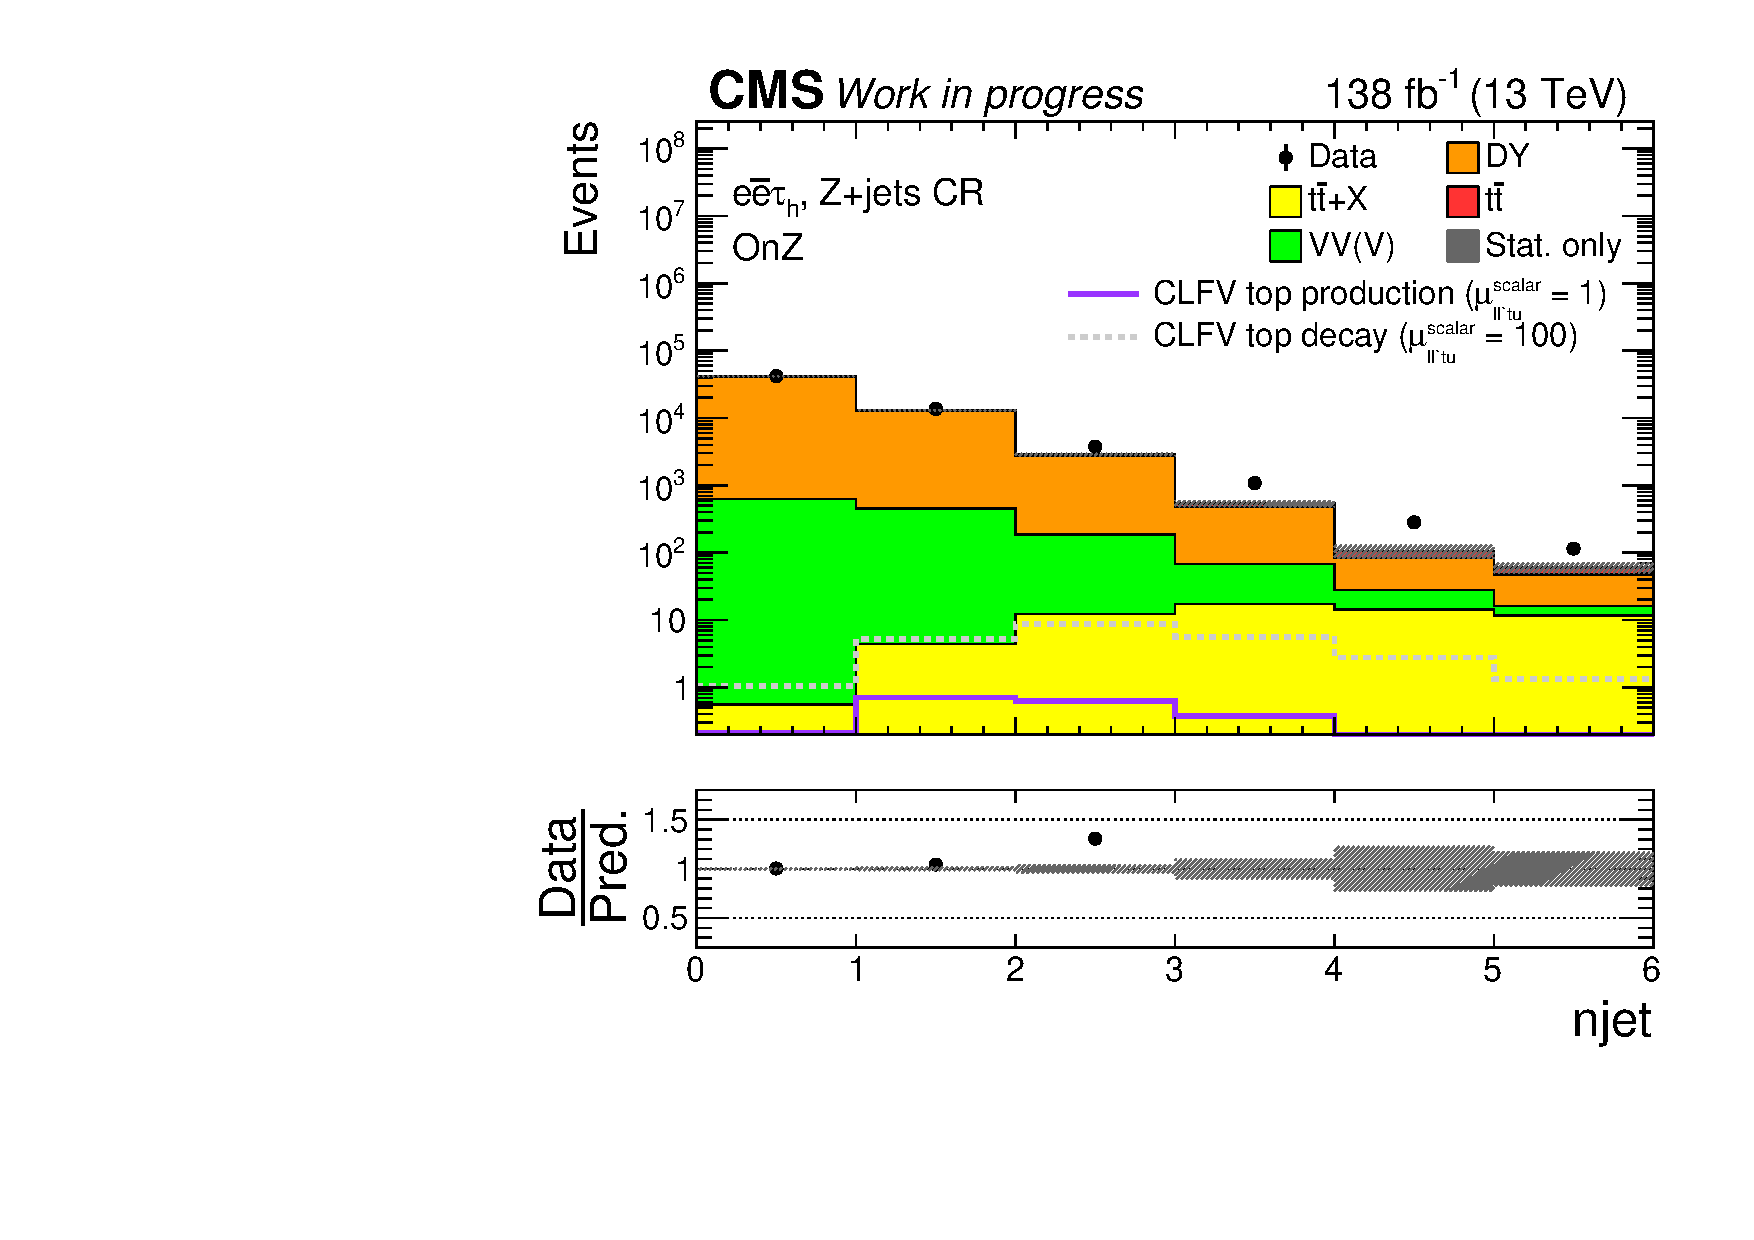
\includegraphics[width=0.48\textwidth]{figures/Part4/Evt/njet_OnZ_ee}&
 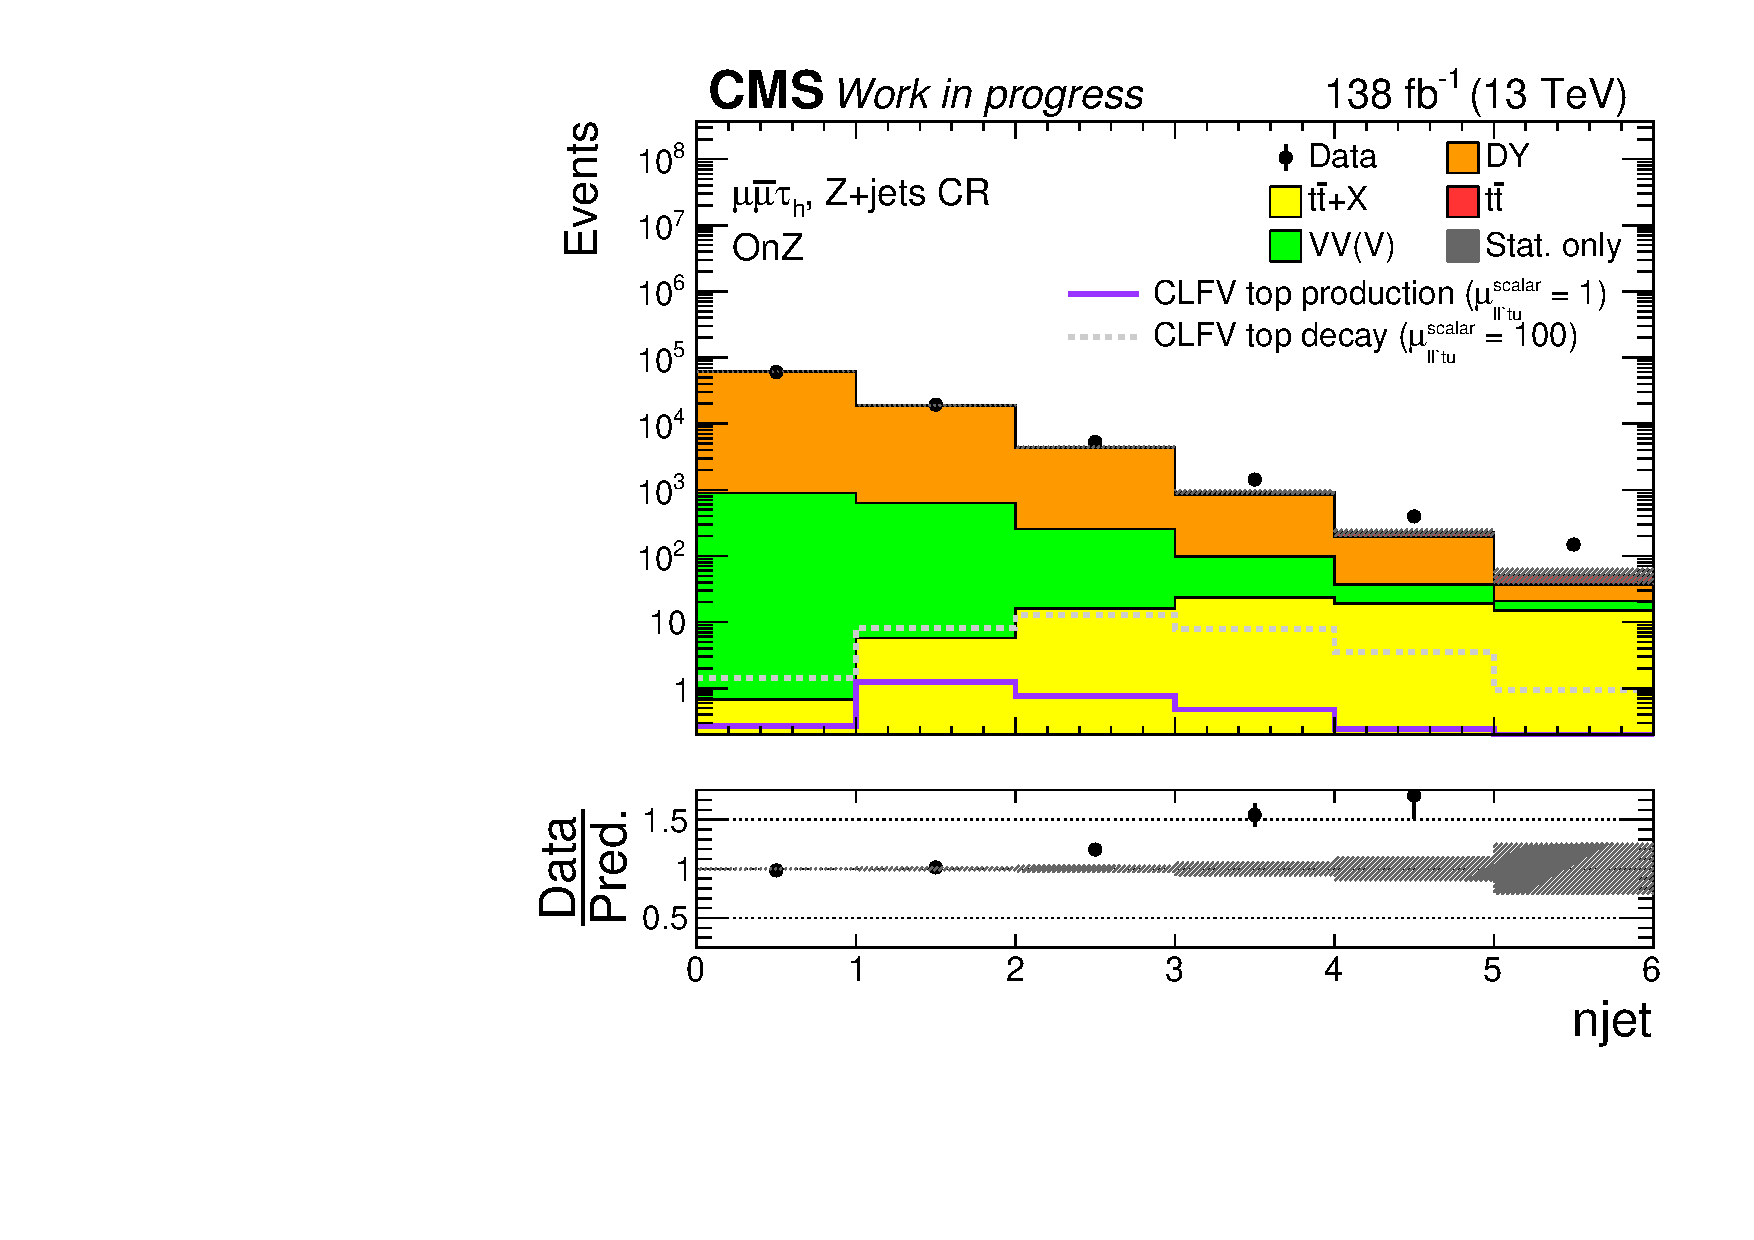
\includegraphics[width=0.48\textwidth]{figures/Part4/Evt/njet_OnZ_mumu}\\
 \end{tabular}
 \caption{XX}
 \label{fig:DY_CR}
 \end{center}
 \end{figure}
\chapter{Expected Sensitivity}
\label{chap:Sensitivity}

Data events in the \acp{SR} of this analysis are still hidden as strategies are still being finalized. Nevertheless, preliminary studies are performed to understand the overall sensitivity, as well as the sensitivity of each event channel. These studies utilize Asimov datasets to reconstruct the likelihood function, which is then used to perform the profile likelihood fit and calculate the upper limits. The Asimov datasets replace data events with background-only template histograms. The one-dimensional profile likelihood fit and upper limit are discussed in \autoref{sec:1d}. The two-dimensional likelihood scan is discussed in \autoref{sec:2d}.
%%%%%%%%%%%%%%%%%%%%%%%%%%%%%%%%%%%%%%%%%%%%%%%%%%%%
%%%%%%%%%%%%%%%%%%%%%%%%%%%%%%%%%%%%%%%%%%%%%%%%%%%%

\section{Upper Limits}
\label{sec:1d}

The one-dimensional likelihood function $\mathcal{L}(\mu, \theta)$ is very similar to the one described in \autoref{sec:PLF} with a few notable differences. Firstly, templates are constructed directly from event yields in search bins as \ac{BDT} is not used in this analysis. Secondly, only statistical uncertainties, luminosity uncertainties, and normalization uncertainties of \ac{MC} samples are considered as other systematic uncertainties are still being evaluated. A 20\% normalization uncertainties are assigned to the normalizations of the $\ttbar$ and \ac{DY} backgrounds as they are considered \emph{fake} tau backgrounds with larger uncertainties. A 10\% uncertainty is assigned to the normalizations of signal and other background processes. Lastly, there are three independent signals contained in one sample, and they are used to construct the likelihood functions separately.

The likelihood function is maximized based on the Asimov datasets. Representative impacts of the nuisance parameters on the likelihood fit are shown in Figure~\ref{fig:Impact_2}.

 \begin{figure}[tbh!]
 \begin{center}
 \begin{tabular}{c}
 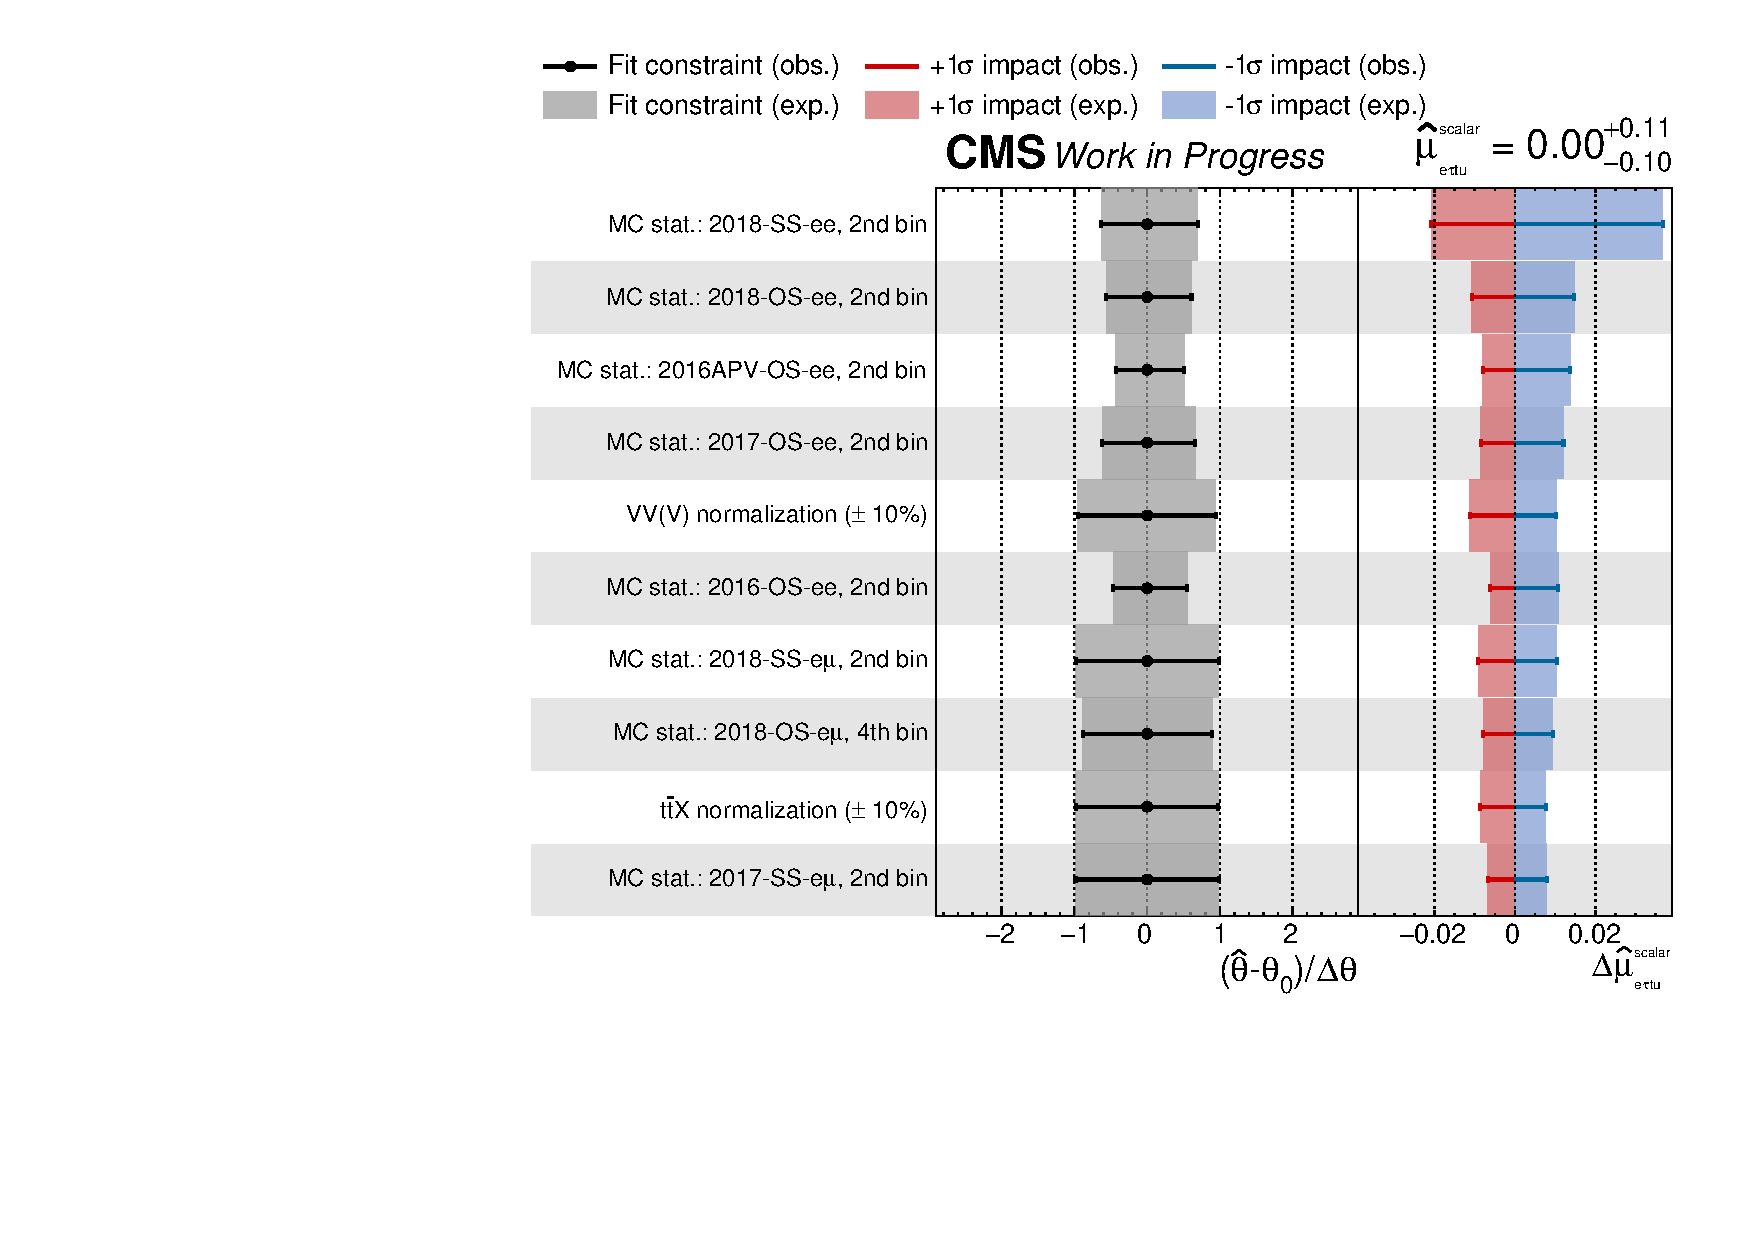
\includegraphics[width=0.9\textwidth]{figures/Part4/Sensitivity/Impact}
 \end{tabular}
 \caption{The nominal value of the expected signal strength $\hat{\mu}$ and its uncertainty is shown in the top right corner. Ranking of the nuisance parameters according to their expected impacts on $\hat{\mu}$ (represented with error bars) is shown in the right panel. Only the 10 nuisance parameters with the largest observed impacts are shown. The impact of each nuisance parameter, $\mathrm{\Delta}\hat{\mu}$, is calculated as the difference between the nominal $\hat{\mu}$ and the value of $\hat{\mu}$ when the corresponding nuisance parameter is fixed to $\hat{\theta}\pm\sigma$, where $\hat{\theta}$ ($\sigma$) is its post-fit value (uncertainty).}
 \label{fig:Impact_2}
 \end{center}
 \end{figure}
 
Using the same limit setting procedure described in \autoref{sec:Limits}, one-dimensional limits at 95\% \ac{CL} can be calculated for each flavor mixing signal. Expected limits on the scalar-like operator involving an up quark are summarized in Table~\ref{tab:limit}.
 
\begin{table}[th]
\sffamily
\centering
\caption{Expected upper limits at 95\% \ac{CL} on \acp{WC} and the branching fractions. The intervals that contain 68\% of the distribution of the expected upper limits are shown in parentheses.}
\resizebox{0.8\linewidth}{!}{%
\begin{tabular}{cccc}
\toprule
CLFV & Event & $\WC{}{\ell\ell^{\prime}\textsf{ut}}/\mathrm{\Lam}^2~(\TeV^{-2})$ & $\mathcal{B} (t \rightarrow \ell\ell^{\prime}\textsf{u}) \times 10^{-6}$ \\
coupling & channel & Exp. (68\% range) & Exp. (68\% range) \\
\midrule
\multirow{4}{*}{$\emut{u}$}& SS-e$\upmu$ & 2.23 (1.84--2.74) & 5.98 (4.07--9.01) \\
& SS-$\upmu\upmu$ & 2.02 (1.66--2.50) & 4.89 (3.30--7.49) \\
& OS-e$\upmu$ & 1.09 (0.91--1.30) & 1.42 (1.00--2.04) \\
& Combined & 1.04 (0.87--1.24) & 1.29 (0.91--1.86) \\
\midrule
\multirow{5}{*}{e$\uptau$ut} & OS-ee & 1.23 (1.04--1.47) & 1.82 (1.30--2.60) \\
 & OS-e$\upmu$ & 0.93 (0.78--1.12) & 1.04 (0.73--1.51) \\
 & SS-ee & 0.69 (0.57--0.85) & 0.58 (0.39--0.87) \\
 & SS-e$\upmu$ & 0.57 (0.48--0.70) & 0.40 (0.27--0.59) \\
 & Combined & 0.49 (0.41--0.59) & 0.29 (0.20--0.42) \\
 \midrule
\multirow{5}{*}{$\upmu\uptau$ut} & OS-$\upmu\upmu$ & 1.14 (0.97--1.36) & 1.56 (1.12--2.22) \\
 & OS-e$\upmu$ & 0.87 (0.73--1.05) & 0.91 (0.64--1.33) \\
 & SS-e$\upmu$ & 0.54 (0.45--0.66) & 0.36 (0.24--0.53) \\
 & SS-$\upmu\upmu$ & 0.48 (0.40--0.60) & 0.28 (0.19--0.43) \\
 & Combined & 0.41 (0.34--0.49) & 0.20 (0.14--0.29) \\
 \bottomrule
\end{tabular}
}
\label{tab:limit2}
\end{table}

%%%%%%%%%%%%%%%%%%%%%%%%%%%%%%%%%%%%%%%%%%%%%%%%%%%%
%%%%%%%%%%%%%%%%%%%%%%%%%%%%%%%%%%%%%%%%%%%%%%%%%%%%

\section{Two Dimensional Likelihood Scan}
\label{sec:2d}

The two-dimensional likelihood function $\mathcal{L}(\mu_1, \mu_2, \theta)$ is constructed by injecting two signals simultaneously. The $\mu_1$ and $\mu_2$ correspond to signal strengths of signals generated in different flavor mixing modes. For a given pair of signal strengths ($\mu_1$, $\mu_1$), nuisance parameters $\theta$ are profile to achieve the maximum likelihood, denoted by $\mathcal{L}(\mu_1, \mu_2, \hat{\theta}_{\mu_1,\mu_2})$. This process is repeated to scan through the $\mu_1$-$\mu_1$ space. The results of the profiled likelihood at each point in $\mu_1$-$\mu_1$ space are then compared with the expected likelihood distribution to locate the boundaries of the 68\% and 90\% ranges, which are shown in Figure~\ref{fig:2DScan}.

 \begin{figure}[tbh!]
 \begin{center}
 \begin{tabular}{ccc}
 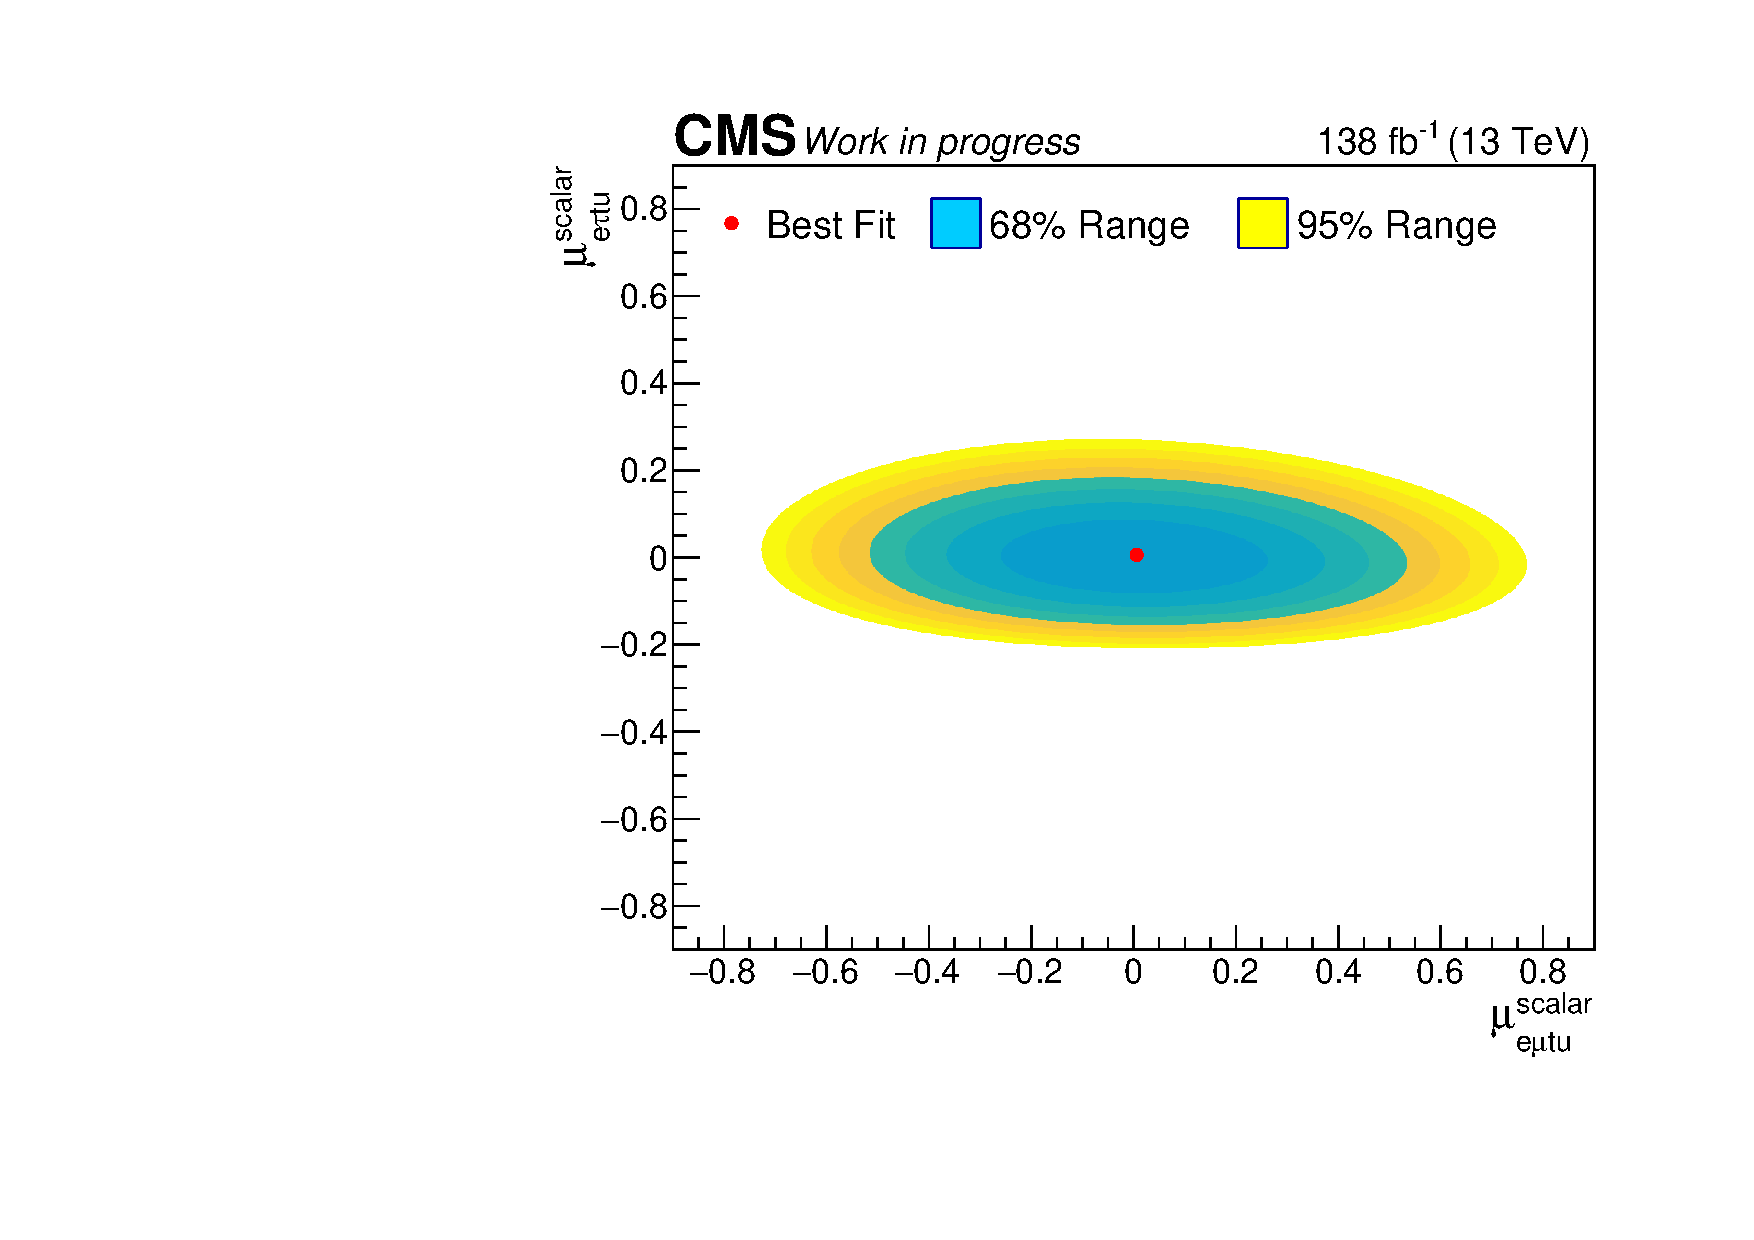
\includegraphics[width=0.33\textwidth]{figures/Part4/Sensitivity/2dScan_emuetau}&
 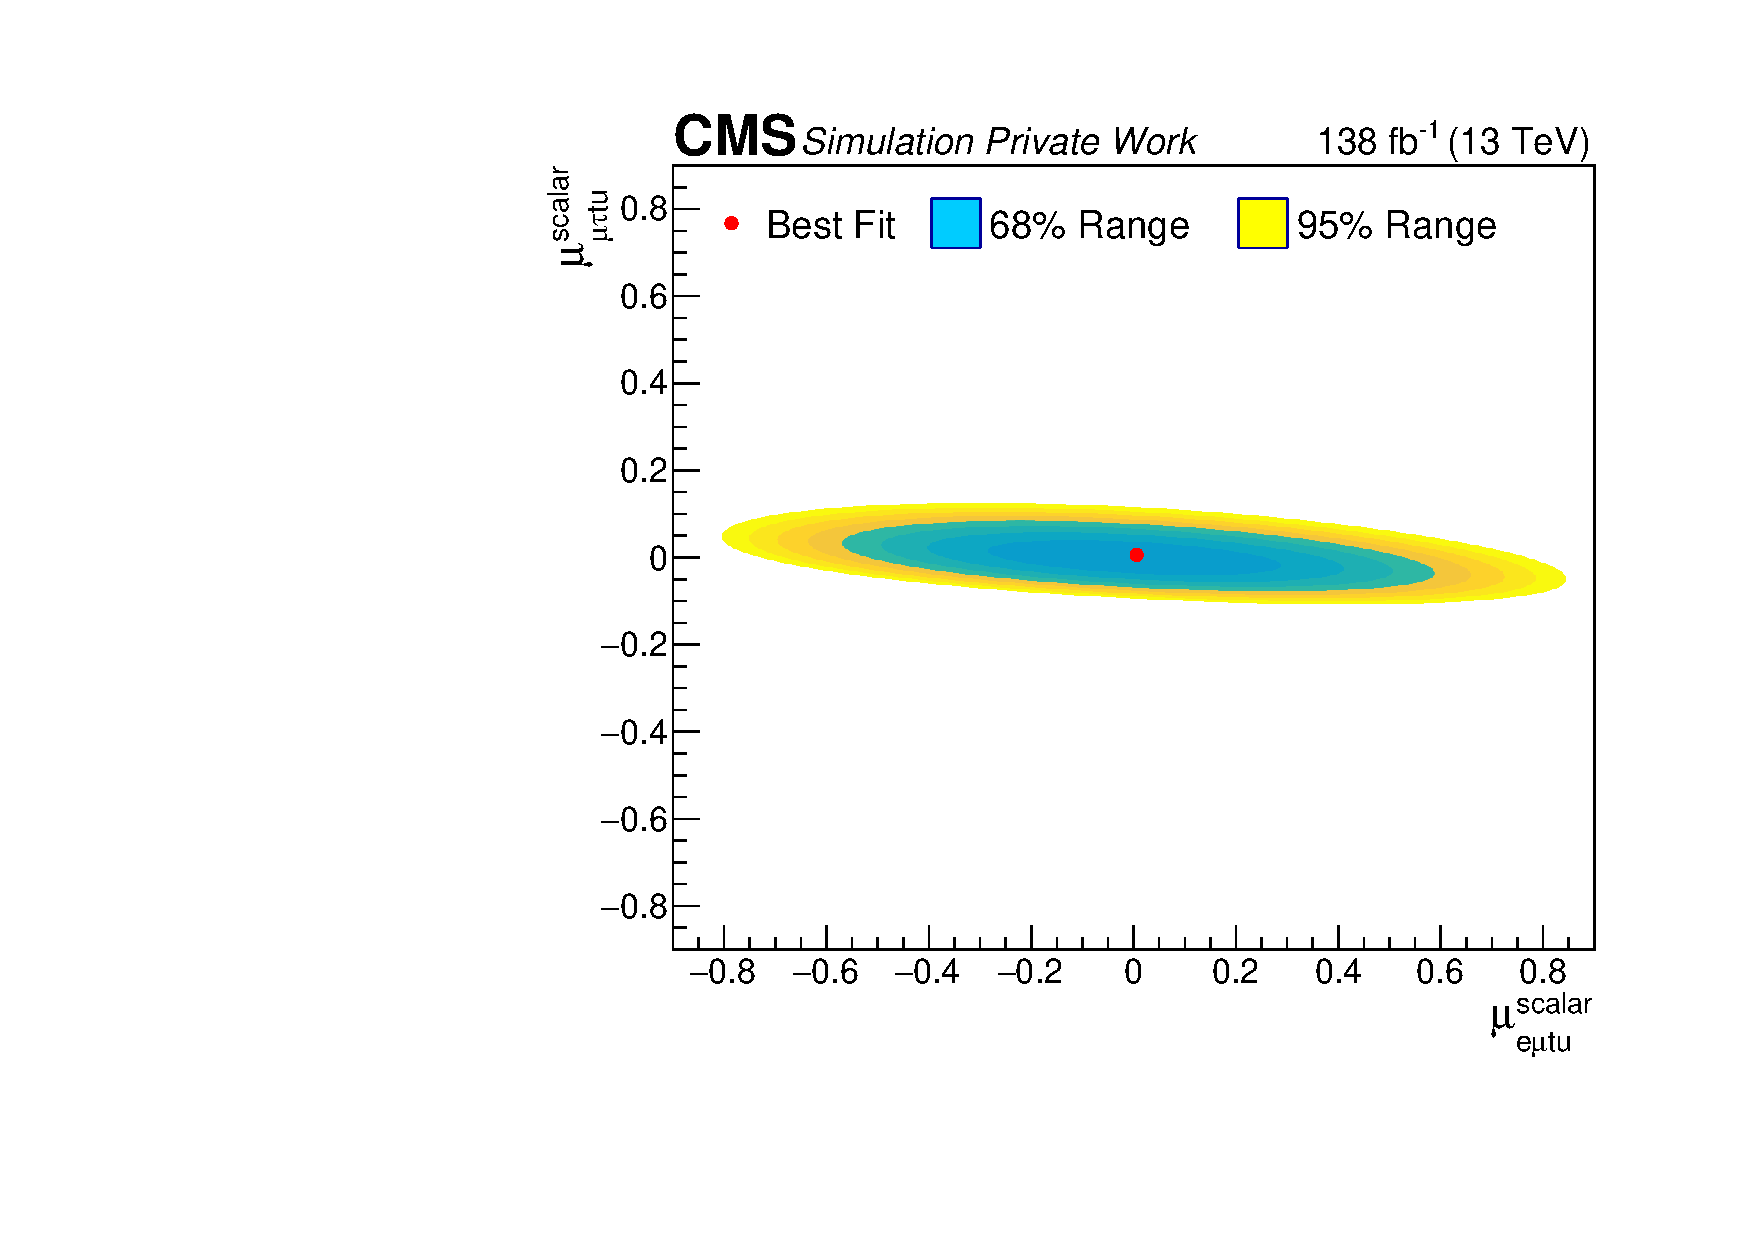
\includegraphics[width=0.33\textwidth]{figures/Part4/Sensitivity/2dScan_emumutau}&
 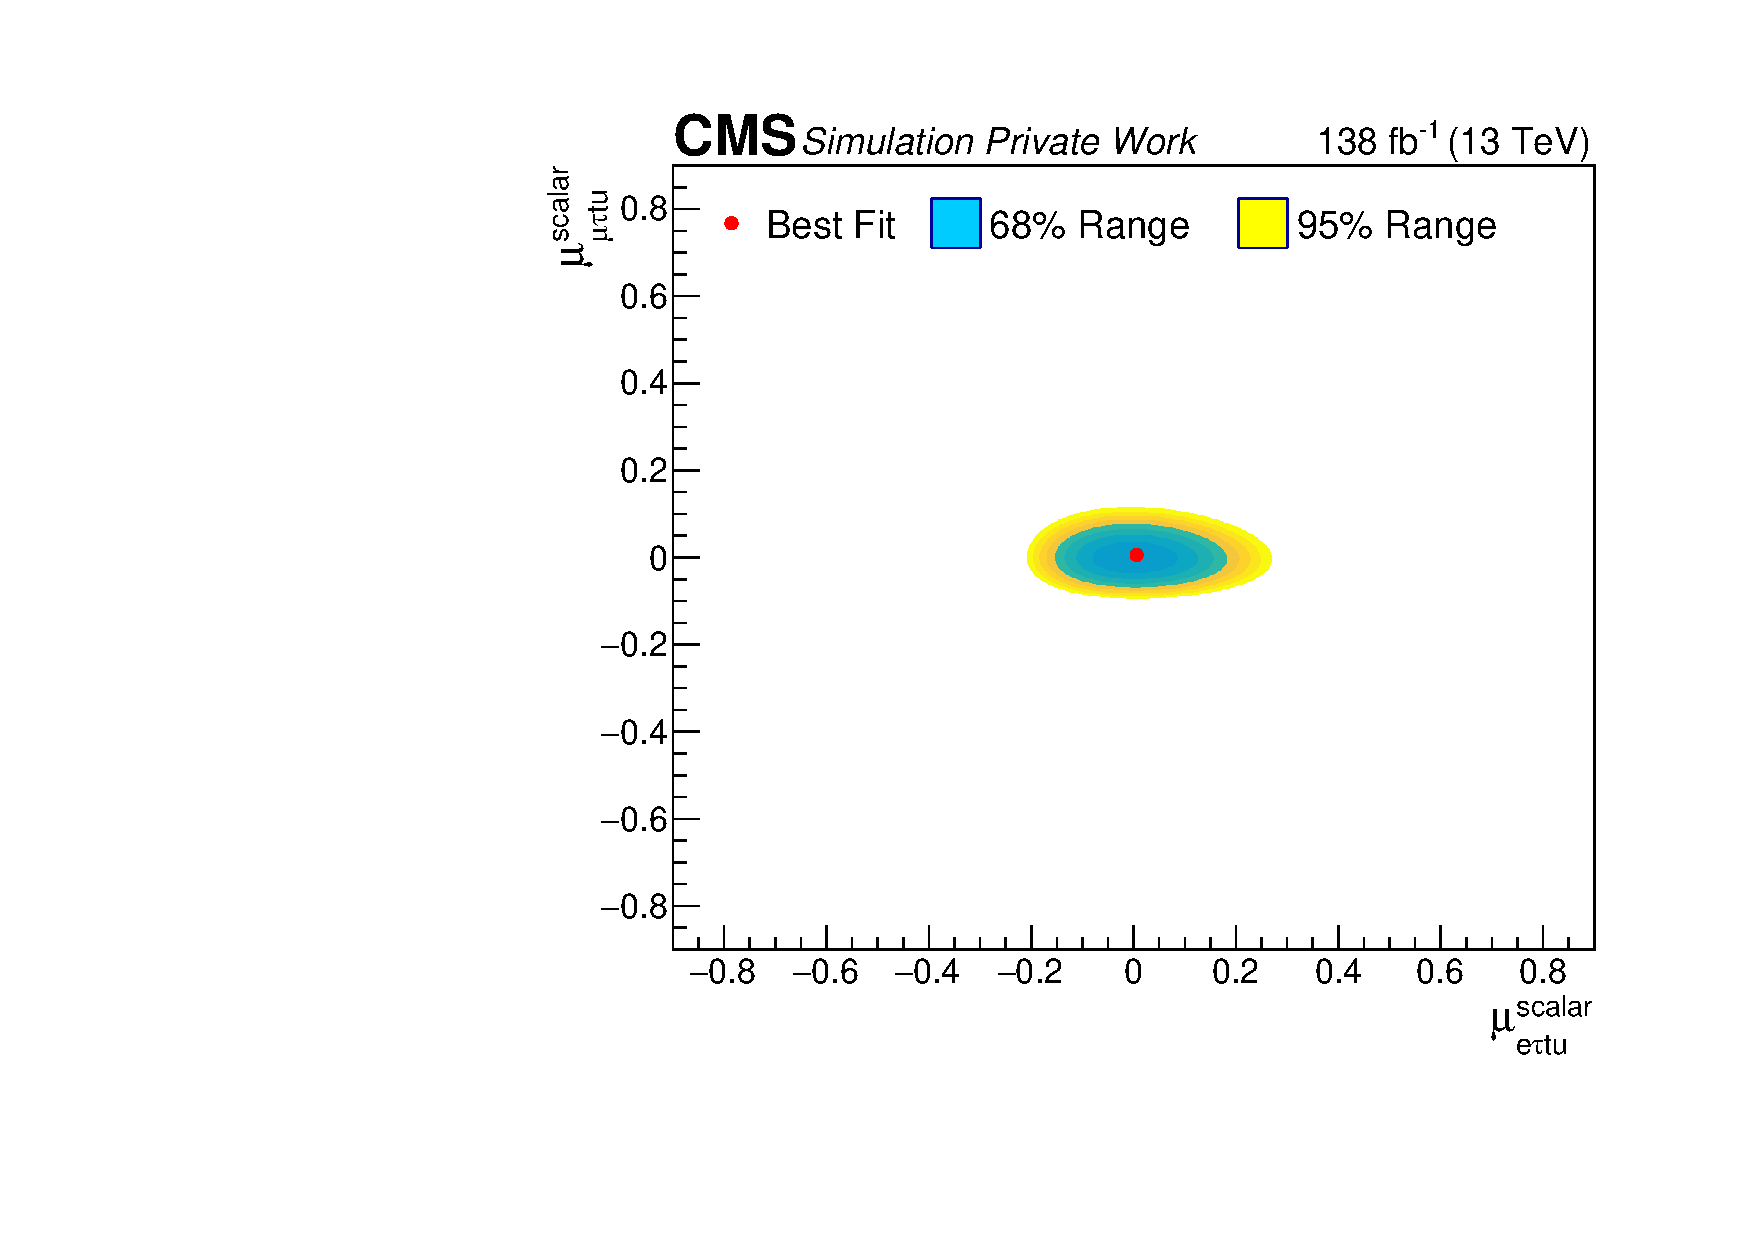
\includegraphics[width=0.33\textwidth]{figures/Part4/Sensitivity/2dScan_etaumutau}\\
 \end{tabular}
 \caption{Two dimensional likelihood scans performed in the e$\upmu$-e$\uptau$ (left), e$\upmu$-$\upmu\uptau$ (middle), and e$\uptau$-$\upmu\uptau$ (right) spaces.}
 \label{fig:2DScan}
 \end{center}
 \end{figure}
